% PLEASE USE THIS FILE AS A TEMPLATE
% Check file iosart2x.tex for more examples

% add. options: [seceqn,secthm,crcready] FC:original:[sw]
\documentclass[sw]{iosart2x}

%\usepackage{dcolumn}

\usepackage{comment} %% utility package: allows multiline comments
\usepackage{xspace}  %% utility package: allows definition of no-argument commands that do not absorb trailing saces
\usepackage{ifthen}  %% utility package: allows for conditionals
\usepackage{xcolor}  %% utility package: colors for temporary comments
\usepackage{enumitem}  %% utility package: change spacing of lists

%%%%%%%%%%%%%%%%%%%%%%%%%%%%%%%%%%%%%%%%%%%%%%%%%%%%%%%%%%%%%%%%%%%%%%%%%%%%%%%%%%%%%%%5
%%%%%%%%%%% Put your definitions here
%%%%% FORMULAS
% COUNTERS
% newcommand for list ox formula environment
\newcommand{\bflist}{\begin{list}{}{\setlength{\topsep}{2mm}\setlength{\partopsep}{0mm}\setlength{\parsep}{0mm}\setlength{\leftmargin}{9mm}\setlength{\labelwidth}{8mm}}}
\newcommand{\eflist}{\end{list}}

% newcommand for labels of axioms, definitions and formulae
\newcommand{\AxLabel}{\textrm{a}}
\newcommand{\DefLabel}{\textrm{d}}
\newcommand{\ExLabel}{\textrm{ex}}
\newcommand{\FmLabel}{\textrm{f}}
\newcommand{\ThrLabel}{\textrm{t}}
\newcommand{\NtsLabel}{{\color{red}\textrm{TODO}}}

% counter and newcommand for numbering formulas
\newcounter{cntax}
\newcommand{\myax}[1]{\refstepcounter{cntax}\begin{small}{\bf \AxLabel\thecntax\label{ax:#1}}\end{small}}
\newcounter{cntdef}
\newcommand{\mydf}[1]{\refstepcounter{cntdef}\begin{small}{\bf \DefLabel\thecntdef\label{def:#1}}\end{small}}
\newcounter{cntfm}
\newcommand{\myex}[1]{\refstepcounter{cntex}\begin{small}{\bf \ExLabel\thecntex\label{ex:#1}}\end{small}}
\newcounter{cntex}
\newcommand{\myfm}[1]{\refstepcounter{cntfm}\begin{small}{\bf \FmLabel\thecntfm\label{for:#1}}\end{small}}
\newcounter{cntthr}
\newcommand{\mythr}[1]{\refstepcounter{cntthr}\begin{small}{\bf \ThrLabel\thecntthr\label{th:#1}}\end{small}}
\newcounter{cntnts}
\newcommand{\mynts}[1]{\refstepcounter{cntnts}\begin{small}{\bf \NtsLabel\thecntnts\label{nts:#1}}\end{small}}

\newcommand{\mytext}[1]{``#1''}

\newcommand{\refax}[1]{({\AxLabel}\ref{#1})}
\newcommand{\refdf}[1]{({\DefLabel}\ref{#1})}
\newcommand{\refex}[1]{({\ExLabel}\ref{#1})}
\newcommand{\reffm}[1]{({\FmLabel}\ref{#1})}
\newcommand{\refth}[1]{({\ThrLabel}\ref{#1})}
\newcommand{\refnt}[1]{({\NtsLabel}\ref{#1})}

%%%%% Predicates styling
%% general style -- purtroppo non funzionano tutti siccome LaTeX fa le storie per le espansioni delle macro, credo
%                 - pero' almeno texttt, textnormal, textbf e textit funzionano; textsc non funziona
\newcommand{\generalStyle}[1]{\texttt{#1}}
%% binary predicate style
\newcommand{\biRel}[3]{\generalStyle{#1}(#2,#3)}
%% monadic predicate style
\newcommand{\uniRel}[2]{\generalStyle{#1}(#2)}
%% monadic predicate (parameterized) style
\newcommand{\uniRelPar}[3]{\generalStyle{#1}_{\generalStyle{#3}}(#2)}
%% binary predicate (parameterized) style
\newcommand{\biRelPar}[4]{\generalStyle{#1}_{\generalStyle{#4}}(#2,#3)}
%% ternary predicate style
\newcommand{\triRel}[4]{\generalStyle{#1}(#2,#3,#4)}
%% 4- predicate style
\newcommand{\fourRel}[5]{\generalStyle{#1}(#2,#3,#4,#5)}
%% 5- predicate style
\newcommand{\fiveRel}[6]{\generalStyle{#1}(#2,#3,#4,#5,#6)}
%% constant style
\newcommand{\cst}[1]{\ensuremath{\mathtt{#1}}}
%% functions 
%\newcommand{\functionIndividual}[1]{\cst{#1}}

%%%%%%% Logic symbols
%% biconditional
\newcommand{\myiff}{\Longleftrightarrow}
%% necessary condition
\newcommand{\myif}{\Longleftarrow \hspace{0.9mm}}
%% sufficient condition
\newcommand{\myfi}{\hspace{0.9mm} \Longrightarrow}

%%%%%%% DOLCE
%% DOLCE style -- Small Caps, ie textsc, non funziona per qualche ragione
\newcommand{\DOLCE}{\textsc{DOLCE}\xspace} %% TODO far si che le macro applichino lo stile :(, perche' textsc non funziona?
\newcommand{\YAMATO}{\textsc{YAMATO}\xspace}
\newcommand{\BFO}{\textsc{BFO}\xspace} 
\newcommand{\GFO}{\textsc{GFO}\xspace} 
\newcommand{\OWL}{\textnormal{OWL}\xspace} 
\newcommand{\TLO}{\textnormal{TLO}\xspace} 


%% DOLCE various predicates
\newcommand{\DOLCEQuality}[1]{\uniRel{Q}{#1}}
\newcommand{\DOLCEEvent}[1]{\uniRel{{E}}{#1}}
\newcommand{\DOLCEDescription}[1]{\uniRel{{DS}}{#1}}
\newcommand{\DOLCEAgent}[1]{\uniRel{{ASO}}{#1}}
\newcommand{\Role}[1]{\uniRel{{Role}}{#1}}
\newcommand{\DOLCERole}[1]{\uniRel{{RL}}{#1}}
\newcommand{\DOLCEState}[1]{\uniRel{{ST}}{#1}}
\newcommand{\DOLCEProcess}[1]{\uniRel{PRO}{#1}}
\newcommand{\DOLCEPerdurant}[1]{\uniRel{{PER}}{#1}}
\newcommand{\DOLCEStative}[1]{\uniRel{{STV}}{#1}}
\newcommand{\DOLCEPhysObj}[1]{\uniRel{{POB}}{#1}}
\newcommand{\DOLCENASO}[1]{\uniRel{{NASO}}{#1}}
\newcommand{\DOLCEConcept}[1]{\uniRel{{CN}}{#1}}

\newcommand{\DOLCEPC}[2]{\biRel{{PC}}{#1}{#2}}
\newcommand{\DOLCEPart}[2]{\biRel{{P}}{#1}{#2}}
\newcommand{\DOLCEOver}[2]{\biRel{{O}}{#1}{#2}}
\newcommand{\DOLCEConstitutes}[2]{\biRel{{constitutes}}{#1}{#2}}
\newcommand{\DOLCEQualityDirect}[2]{\biRel{qt}{#1}{#2}}
\newcommand{\DOLCEQualeDirect}[2]{\biRel{{ql}}{#1}{#2}}
\newcommand{\DOLCECLby}[2]{\biRel{CL}{#1}{#2}}
\newcommand{\DOLCEPRE}[2]{\biRel{PRE}{#1}{#2}}

\newcommand{\DOLCESum}[3]{\triRel{Sum}{#1}{#2}{#3}}
\newcommand{\DOLCECLbyPar}[3][]{\biRelPar{{CL}}{#2}{#3}{#1}}

%%%% Additional predicates
\newcommand{\RelationalQualityClass}{\generalStyle{relationalQt}}
\newcommand{\CapabilityClass}{\generalStyle{Capability}}
\newcommand{\CapacityClass}{\generalStyle{Capacity}}

\newcommand{\TechArt}[1]{\uniRel{TechArt}{#1}}
\newcommand{\Component}[1]{\uniRel{Component}{#1}}
\newcommand{\Capability}[1]{\uniRel{Capability}{#1}}
\newcommand{\PumpingCapability}[1]{\uniRel{PumpingCapability}{#1}}
\newcommand{\PumpingProcess}[1]{\uniRel{PumpingProcess}{#1}}
\newcommand{\BehaviourAbstract}[1]{\uniRel{AbstBeh}{#1}}
\newcommand{\BehaviourConcrete}[1]{\uniRel{Behaviour}{#1}}
\newcommand{\Capacity}[1]{\uniRel{Capacity}{#1}}
\newcommand{\RelationalQuality}[1]{\uniRel{relationalQt}{#1}}
\newcommand{\IntrinsicQuality}[1]{\uniRel{intrinsicQt}{#1}}
\newcommand{\Goal}[1]{\uniRel{Goal}{#1}}
\newcommand{\StateVariable}[1]{\uniRel{StateVariable}{#1}}
\newcommand{\System}[1]{\uniRel{System}{#1}}
\newcommand{\StateVariableCondition}[1]{\uniRel{SystemCond}{#1}}
\newcommand{\Method}[1]{\uniRel{Method}{#1}}

\newcommand{\FunctionSys}[1]{\uniRelPar{Function}{#1}{Sys}}
\newcommand{\FunctionEng}[1]{\uniRelPar{Function}{#1}{Eng}}

\newcommand{\inheres}[2]{\biRel{inheres}{#1}{#2}}
\newcommand{\specificallyDependsOn}[2]{\biRel{dependsOn}{#1}{#2}}
%SD(x,y) , (∃t(PRE(x,t))∧∀t(PRE(x,t) → PRE(y,t))) (Specific Const. Dep.)
\newcommand{\founded}[2]{\biRel{\foundedTerm{passive}}{#1}{#2}}

\newcommand{\contextOf}[2]{\biRel{contextOf}{#1}{#2}}
\newcommand{\causallyContr}[2]{\biRel{causalContr}{#1}{#2}}
\newcommand{\participatedAsDoer}[2]{\biRel{participatedAsDoer}{#1}{#2}}
\newcommand{\participateAsDoer}[2]{\biRel{participatesAsDoer}{#1}{#2}}
\newcommand{\participateAsFlow}[2]{\biRel{participatesAsFlow}{#1}{#2}}
\newcommand{\behaviourOf}[2]{\biRel{behaviourOf}{#1}{#2}}
\newcommand{\goalOf}[2]{\biRel{goalOf}{#1}{#2}}
\newcommand{\external}[2]{\biRel{externalTo}{#1}{#2}}
\newcommand{\internal}[2]{\biRel{internalTo}{#1}{#2}}
\newcommand{\mainFunction}[2]{\biRel{mainFunction}{#1}{#2}}
\newcommand{\subFunction}[2]{\biRel{subFunction}{#1}{#2}}
\newcommand{\playAs}[2]{\biRel{playAs}{#1}{#2}}

\newcommand{\partTA}[2]{\biRelPar{P}{#1}{#2}{TA}}
\newcommand{\partS}[2]{\biRelPar{P}{#1}{#2}{Sys}}
\newcommand{\describedBy}[2]{\biRelPar{describedBy}{#1}{#2}{Cap}}
\newcommand{\realizedIn}[2]{\biRelPar{realizedIn}{#1}{#2}{Beh}}
\newcommand{\foundedCapab}[2]{\biRelPar{founded}{#1}{#2}{Cpb}}
\newcommand{\foundedROLE}[2]{\biRelPar{\foundedTerm{passive}}{#1}{#2}{RL}}

\newcommand{\participateAsDoerTemp}[3]{triRel{participatesAsDoer}{#1}{#2}{#3}}
\newcommand{\behSum}[3]{\triRel{Sum}{#1}{#2}{#3}}
\newcommand{\DOLCEQualeTer}[3]{\triRel{ql}{#1}{#2}{#3}}

%% Fnctional Basis Thingies
\newcommand{\Flow}[1]{\uniRel{Flow}{#1}}
\newcommand{\flowOf}[2]{\biRel{flowOf}{#1}{#2}}
\newcommand{\Energy}[1]{\uniRel{Energy}{#1}}
\newcommand{\Material}[1]{\uniRel{Material}{#1}}
\newcommand{\Signal}[1]{\uniRel{Signal}{#1}}
\newcommand{\inp}[2]{\biRel{inp}{#1}{#2}}
\newcommand{\out}[2]{\biRel{out}{#1}{#2}}
\newcommand{\ABSum}[3]{\triRel{ASum}{#1}{#2}{#3}}

%% decomposition
%\newcommand{\decom5}[5]{\fiveRel{comp}{#1}{#2}{#3}{#4}{#5}}
\newcommand{\decom}{\generalStyle{decomp}}

%%%% First time keyword - usare quando una parola chiave [] menzionata per la prima volta
\newcommand{\firstTimeKeyWord}[1]{\textit{#1}}

%%%% Terminology - termini introdotti dall'articolo, potenzialmente questionabili, da modificare facilmente
%%%%%% Terminologia

%% individual quality founds capability
\newcommand{\foundedTerm}[1]{%
  \ifthenelse{\equal{#1}{passive}}{founded}{%
    \ifthenelse{\equal{#1}{verb}}{found}{%
      \ifthenelse{\equal{#1}{gerund}}{founding}{%
        ERROR!%
      }%
    }%
  }%
}  

%% changings of state variables
\newcommand{\stateVarCond}[1]{%
  \ifthenelse{\equal{#1}{fullSingular}}{system condition}{%
    \ifthenelse{\equal{#1}{shortSingular}}{condition}{%
      \ifthenelse{\equal{#1}{fullPlural}}{system conditions}{%
        \ifthenelse{\equal{#1}{shortPlural}}{conditions}{%
          ERROR!%
        }%
      }%
    }%
  }%
}  


%% single quotes
\newcommand{\quotes}[1]{`#1'}
%%%%%%%%%%%%%%%%%%%%%%%%%%%%%%%%%%%%%%%% miscellanea
%%%%%% The following 4 lines are from https://tex.stackexchange.com/questions/287081/how-to-prevent-a-linebreak-before-align-equation-environment-in-itemize/287091#287091
\newcommand{\myalignspaceskip}{
 \abovedisplayskip=-\baselineskip
 \belowdisplayskip=0pt
 \abovedisplayshortskip=-\baselineskip
 \belowdisplayshortskip=0pt}
%%%%%% Commenti
\newcommand{\TODO}[1]{{\color{red} #1}}
\newcommand{\TODOinline}[1]{{\color{red} #1}}
%\newcommand{\TODO}[1]{\nb{#1}}
%red comment in the margin
\newcommand{\nb}[1]{\textcolor{red}{$|$}\marginpar{\parbox{22mm}{\scriptsize\raggedright\textcolor{red}{#1}}}}
% to comment away a small text
\newcommand{\myComment}[1]{}

%%%%%%%%%%%%%%%%%%%%%%%%%%%%%%%%%%%%%%%%
%%%%%%%%%%% End of definitions
%%%%%%%%%%%%%%%%%%%%%%%%%%%%%%%%%%%%%%%%%%%%%%%%%%%%%%%%%%%%%%%%%%%%%%%%%%%%%%%%%%%%

\pubyear{0000}
\volume{0}
\firstpage{1}
\lastpage{1}

\begin{document}

\begin{frontmatter}

%\pretitle{}
\title{About functions, behaviours, and capabilities in formal ontology and engineering}
\runtitle{Running head title}
%\subtitle{}

% For one author:
%\author{\inits{N.}\fnms{Name1} \snm{Surname1}\ead[label=e1]{first@somewhere.com}}
%\address{Department first, \orgname{University or Company name},
%Abbreviate US states, \cny{Country}\printead[presep={\\}]{e1}}

% Two or more authors:
\begin{aug}
\author[A]{\inits{N.}\fnms{Name1} \snm{Surname1}\ead[label=e1]{first@somewhere.com}%
\thanks{Corresponding author. \printead{e1}.}}
\author[B]{\inits{N.N.}\fnms{Name2 Name2} \snm{Surname2}\ead[label=e2]{second@somewhere.com}}
\author[B]{\inits{N.-N.}\fnms{Name3-Name3} \snm{Surname3}\ead[label=e3]{third@somewhere.com}}
\address[A]{Department first, \orgname{University or Company name},
Abbreviate US states, \cny{Country}\printead[presep={\\}]{e1}}
\address[B]{Department first, \orgname{University or Company name},
Abbreviate US states, \cny{Country}\printead[presep={\\}]{e2,e3}}
\end{aug}

%\begin{review}{editor}
%\reviewer{\fnms{First} \snm{Editor}\address{\orgname{University or Company name}, \cny{Country}}}
%\reviewer{\fnms{Second} \snm{Editor}\address{\orgname{First University or Company name}, \cny{Country}
%    and \orgname{Second University or Company name}, \cny{Country}}}
%\end{review}
%\begin{review}{solicited}
%\reviewer{\fnms{First} \snm{Solicited reviewer}\address{\orgname{University or Company name}, \cny{Country}}}
%\reviewer{\snm{anonymous reviewer}}
%\end{review}
%\begin{review}{open}
%\reviewer{\fnms{First} \snm{Open Reviewer}\address{\orgname{University or Company name}, \cny{Country}}}
%\end{review}

\begin{abstract}
%% NOTA (estratti dal testo della call):
%... industrial environments where machines are designed to smoothly interact between themselves and with humans via knowledge models. 
%At the same time, however, 
%practitioners and stakeholders lack methodologies and guidelines to reliably develop, use or integrate (existing) ontologies ...
%% (elenco alcuni temi)
%-...
%-Ontologies for knowledge representation and reasoning about topics relevant for industrial engineering (e.g., products, processes, manufacturing resources, requirements and capabilities, etc.).
%-Ontology-based patterns for industrial engineering knowledge representation.
%-ethodologies, methods, and techniques targeted to industrial contexts supporting the development, modularization, extension, and evolution of ontologies.
%-Literature review of existing ontologies for industrial engineering, including structured comparisons.
%-Experiences with the use of top-level ontologies (e.g. BFO, DOLCE, ISO 15926, among others) in industrial engineering.
%-Experiences with research and application initiatives such as OntoCommons, the Industry Ontologies Foundry (IOF), and the UK National Digital Twins.
%
%
%% NOTA (estratti dal file iosart2x.pdf)
%...
%� The use of first persons (i.e., �I�, �we�, �their�, possessives, etc.) should be avoided, and can preferably be
%expressed by the passive voice or other ways. This also applies to the Abstract.
%� A research paper should be structured in terms of four parts, each of which may comprise of multiple sections:
%   * Part One is problem description/definition, and a literature review upon the state of the art.
%   * Part Two is methodological formulation and/or theoretical development (fundamentals, principle and/or ap-
%     proach, etc.).
%   * Part Three is prototyping, case study or experiment.
%   * Part Four is critical evaluation against related works, and the conclusion.
%In any article it is unnecessary to have an arrangement statement at the beginning (or end) of every (sub-) section.
%Rather, a single overall arrangement statement about the whole paper can be made at the end of the Introduction
%section. ...
%
%
% old abstract
\begin{comment} 
In both applied ontology and engineering, a rich portion of the literature has researched ways to represent the functionality of engineering systems. 
Such a topic is of fundamental importance, since it is through teleological causal reasoning, which gives birth to functions, that domain experts build mental 
models of machines and the like. 
Furthermore, functionality is important throughout the whole lifecycle of any product, being used from the design phase to any eventual
diagnosis activity. 

A vast amount of work has already been done; even so the literature has not settled on a unique and well-defined methodology. 
This work develops preliminary steps towards an ontological description of functions and related concepts, such as behaviour and capability.
This is accomplished through a conceptual analysis of the fundamental notions related to functionality, carried out using the top-level ontology \cite{borgoDOLCEDescriptiveOntology2022}. 
A formal description is given in \TODOinline{first order logic/???} \OWL, and some examples are worked through.
\end{comment}
In both applied ontology and engineering, functionality is a well-researched topic, since it is through teleological causal reasoning that domain experts build mental models of engineering systems, giving birth to functions. 
These mental models are important throughout the whole lifecycle of any product, being used from the design phase up to any eventual diagnosis activity. 
A vast amount of work to represent functions has already been carried out, even so the literature has not settled on a shared and well-defined methodology. 
This work develops preliminary steps towards an ontological description of functions and related concepts, such as behaviour, capability, and capacity.
A conceptual analysis of such notions is carried out using the top-level ontology DOLCE as a framework. 
The ensuing logical theory is formally described in both first order logic and OWL, and some examples are worked through\TODO{check what really is done}, showing how ontological concepts can model major aspects of engineering products in applications.
In particular, it is shown how the distinction between abstract functions and implementation methods explains the difference between capabilities and capacities of a product. \TODO{is it though?}
\end{abstract}

\begin{keyword} 
    %% NOTA
    % ... Please include 3-7 keywords below the abstract of your manuscript. ... 
\kwd{Ontology}
\kwd{Function}
\kwd{Behaviour}
\kwd{Capability}
\end{keyword}

\end{frontmatter}

%%%%%%%%%%%%%%%%%%%%%%%%%%%%%%%%%% ELENCO Di TODOS
%% TODO we give 3 contribution 1 review 2 some distinction et formaliz 3 la roba capab vs capac
%% TODO check that "the reference number is not used at the beginning of a sentence" or " integrate the authors’ names into the text,"
%% TODO dire che metodo = label per composizione di ??comportmaenti??funzioni?? e dire che è meglio che rispetto a FR
%% TODO observer --> agent
%% TODO Ruolo in DOLCE
%% TODO Occurrent vs perdurant
%% TODO cambiare la definizione di behavior come abberbio per SB
%% TODO SB si è contraddetto dicendo di fissare capab vs capacity all'inizio, poi ha detto che il contributo del paper era distinguerle in base alla differenza tra funz ont. vs ing.. Come risolvere?
%% TODO inserire FBS modeler di Umeda (e suo sviluppo: vedi Umeda 2015) e confrontare con Erden 2008
%% TODO sostituire 'I', 'us', 'we', 'our', etc. con costrutti alternativi, come da linee guida stilistiche
%% TODO aggiustare l'uso indiscriminato del genitivo sassone
%% TODO controllare l'uso delle forme ortografiche inglesi o americane, che siano costanti. E.g. 'behaviOUR', 'fomaliSation', 'axiomatiSation', in generale -'Sation' etc.
%%%%%%%%%%%%%%%%%%%%%%%%%%%%%%%%%% FINE TODOS

%%%%%%%%%%% The article body starts:

\section{Introduction}\label{sec:intro}
%% TODO Rivedere dopo il resto del materiale è completato.

%% Introdurre lettore a contesto-->Partire da descrizione contesto in cui ci poniamo: Integrare visuone funzionale solida ont. in visione in ingegneria, in generale. Varie teorie da consolidare
% introduzione 
%% TODO questo paragrafo è insulso --> modificare
Functionality is a concept that has interested engineers as well as philosophers and applied ontologists. 
% esemplificazione
It is referenced whenever engineers and scientists discuss the goals of systems, both natural and artificial.%, therefore, it has great importance in applied and theoretical research alike. 
For example, engineers commonly use functions in order to design \cite{pahl_engineering_2007} and diagnose devices \cite{larssonDiagnosisBasedExplicit1996}, while philosophers discuss the nature of functions themselves \cite{cumminsFunctionalAnalysis1975}.

%% Dire problemi che ci poniamo: quali problemi in questo ambito
% problemi
Despite the high amount of attention given to this topic, some problems have not been settled yet. 
For instance, the terminology used is quite ambiguous and words such as \firstTimeKeyWord{capability}, \firstTimeKeyWord{capacity}, \firstTimeKeyWord{behavior}, or \firstTimeKeyWord{function} itself have many different meanings \cite{borgoCapabilitiesCapacitiesFunctionalities2021, erdenReviewFunctionModeling2008}, and are characterized differently, if at all\myComment{, depending on the author}.
Moreover, the study of \firstTimeKeyWord{functional decomposition}, that is, the division of functions into sub-functions, is often addressed in the literature, but rarely formalized.
Functional decomposition is carried out by designers to \quotes{solve} the main-function, that is, to move one step further in the design process, towards the implementation of the functional requirements into a concrete physical system.
Of course, functional decomposition is not limited to the design of engineering systems. 
In fact, during the teleological analysis of a system, artificial or natural, domain experts speak about functions of both the system and its parts.
Therefore, one is always confronted with the problem of how simpler functions contribute to coarser granularity functions, so that functional decomposition is ubiquitous. %, which themselves push the system towards the desired state.
Since in engineering there exist standard ways to execute functions\footnote{For example, the use of gearboxes made in a certain way in order to increase or reduce angular velocity. Another example: a brushless electric motor may be understood as the class subsuming all models of brushless electric motors, but it can also be recognized as a method by which electric energy can be converted to torque.}, we can speak of \firstTimeKeyWord{engineering methods}\footnote{If the method is not standard, say if it has just been introduced, we still call it an engineering method. In fact, in such a case, the term can refer to the principles and theories, which are shared among engineers, that the implementation follows.}, or solutions \cite{pahl_engineering_2007}, or ways of functional achievement \cite{kitamuraOntologicalModelDevice2006}. \myComment{, the last two terms taken from \cite{pahl_engineering_2007} and \cite{kitamuraOntologicalModelDevice2006} respectively}   

%% Si elencano research question (quali problemi aperti a cui rispondere)
% research questions: 
% 1 - funzioni ont. vs funzioni ing.
% 2 - funzioni vs metodi
% 3 - in un modo formale
% 4 - ???
This paper builds on previous research, especially \cite{borgoCapabilitiesCapacitiesFunctionalities2021} and \cite{mizoguchiUnifyingDefinitionArtifact2016}, to discuss what functionality and related concepts are, in a formal way. 
The formal languages used are first order logic and \OWL; additionally, to give a clear ontological grounding for our formalisation, we use the top-level ontology \DOLCE\footnote{The interested reader can find a complete and in-depth presentation of \DOLCE in \cite{masoloWonderWebDeliverableD182003} and its application in use cases in \cite{borgoDOLCEDescriptiveOntology2022}.} as reference. 
Moreover, we will discuss the relation between functions as objects independent of any implementations, which we call \firstTimeKeyWord{ontological functions}, and functions as objects related to an execution method, which we call \firstTimeKeyWord{engineering function}\TODO{<--controllare questa caratterizzazione}.
Such a dichotomy between functions will be leveraged to explain a possible way to distinguish between capabilities and capacities of engineering artifacts.   
%[sentence moved for better theme linking]The paper uses a formal approach, both in first order logic and in \OWL, so that our proposal is as unambiguous as possible. 
%To facilitate the formalisation and to give a clear ontological grounding for the discussed concepts, the top-level ontology \DOLCE is used as reference.   

% structure statement
The structure of the paper is as follows. A review of the literature about functionality that is particularly relevant for this work is presented in Section \ref{sec:review}. 
Section \ref{sec:DOLCE} describes key concepts of \DOLCE. These are exploited in Section \ref{sec:capabilitiesEtc} for the discussion of capabilities, capacities, behaviors, and functions. This section proposes also a formal interpretation of ontological and engineering functions in first order logic. 
Finally, we give a preliminary ontology in the \OWL language\TODO{[nota: nell'abstract si parla di OWL e FOL. FC: aggiunto "FOL" frase prima, ricontrollare comunque]} in Section \ref{sec:appendice}, before drawing our conclusions in Section \ref{sec:conc}. 

%% Review letteratura
\section{Literature review\label{sec:review}}%
% review parte 1: introduzione ai lavori principali in letteratura sulle funzioni in generale: cosa è una funzione, che vocabolari sono usati
Due to strong practical interests, a vast literature about functionality has been developed within engineering. 
We limit ourselves to a brief review. The reader interested in a more in depth analysis can refer to other works like~\cite{erdenReviewFunctionModeling2008} in engineering and \cite{artigaNewPerspectiveOnFunctions} in applied ontology.

%% TODO frase molto lunga
Fundamental works about functionality are, for example, De Kleer's \cite{de_kleer_how_1984, kleer_qualitative_1984}, which outline foundational principles such as the locality of functions (functions of a component should refer only to neighboring entities) and the \quotes{no function in structure} principle (structural models should not contain teleological information); and Pahl \& Beitz's \cite{pahl_engineering_2007}, which describes functions as black-box transformations applied to input flows, divides functions based on the property of the flow acted upon (e.g., quantity, type, position, etc.), and discusses function decomposition (that is, how to achieve a given function through a structure of adequate sub-functions).

In \cite{pahl_engineering_2007} Pahl \& Beitz explain also how designers can start from a generic function and implement it with solutions based on different physical principles. 
Then, they reference many design catalogues, for example Roth's \cite{rothKonstruierenMitKonstruktionskatalogen2000}, which tabulate solutions and classify them along different criteria.
In the context of design catalogues, functions and solutions exists along the same abstract-concrete axis, and differ by the \quotes{degree of embodyment}. 
Thereby the most abstract functions, called \quotes{generally valid functions}, are the most useful criteria to classify solutions in a product independent way. 

The definition of functions as (selected) actions on flows is the most common type encountered in the engineering literature, for example Chandrasekaran \& al. \cite{chandrasekaranFunctionalRepresentationDesign1993} speak of \quotes{intended input-output relations}, and many vocabularies were proposed in order to standardize function terminology. 
The proposed vocabularies range from Keuneke's short four terms list (toMake, toMantain, toPrevent, and toControl) \cite{keuneke_device_1991}, to bigger vocabularies built using complex algorithms, as Kitamura \& al.'s \cite{kitamuraFunctionalConceptOntology2002a}. 
A common and often referred to example is Stone \& Wood's Functional Basis \cite{hirtz_functional_2002, stone_development_2000}, that gives terms for actions and flows on a three-levels taxonomy described in natural language.

The literature about the use of such vocabularies has not settled yet and, currently, different lines of research are being pursued, such as behavioural simulation of a system from the functional model \cite{kurtogluGraphBasedFaultIdentification2008} or formal description and automatic construction of the functional model itself \cite{gill_logic_2021,kurtoglu_automating_2010}.

%These vocabularies equate functions to transformations of objects, thus using verbs or verbs-objects[nouns] pair as terms. 
% review parte 2: funzioni parte oggettiva vs soggettiva --> introduzione a behaviour
It is generally recognized that functionality depends on the intention of an agent, a typical example being the designer's one \cite{kitamuraOntologyBasedFunctionalKnowledgeModeling2004}, also called \quotes{design rationale} \cite{chandrasekaranFunctionalRepresentationDesign1993}. 
Thus, functions are not objective, at least not completely. 
Then, it is natural to wonder what in a function is fully objective. Behaviour, intended as what a device does, as determined by physical laws, is usually the answer.    

%Also for the term behaviour we have no universally shared definition, but such a concept is usually countraposed to \quotes{function}. Some authors say that behaviour is what  

Even the term behaviour is used ambiguously and without any universally shared definition. 
The ambiguity has such consequences so that some authors classified the multiple uses of behavior in engineering literature: 
Kitamura \& al. \cite{kitamuraOntologyBasedFunctionalKnowledgeModeling2004} determine four types of device behaviour\footnote{They explicitly exclude static behaviours such as supporting, though.}, depending on whether the device changes the state of another device, its own state, or the state of one of its operands. Within the second behavior type are distinguished two additional cases: the operand can either stay in the same position or `move' from the input to the output ports (the latter case is called \firstTimeKeyWord{B1 behavior}).
Instead, in \cite{chandrasekaranFunctionDeviceRepresentation2000}, Chandrasekaran \& Josephson divide behaviours mainly depending on their time duration (instant, interval, or unspecified).

%\TODO{vedere se inserire qui discorso differenza tra behaviour astratti e concreti--->nope(?): non inserire}

The link between function and behaviour generally reflects the duality between objectivity and intentionality: some authors state that behaviour is what a device does, whilst function is what a device is for \cite{kleer_qualitative_1984}, others focus on describing behaviour as a sequence of state changes and functions as abstractions of behaviours with a goal in mind \cite{umedaFunctionBehaviourStructure1990}.  
In \cite{sasajimaFBRLFunctionBehavior1995, sasajimaInvestigationDomainOntology1994}, Sasajima \& al. state that function is made from behaviour plus additional teleological information called \quotes{functional topping}.
Specifically, the functional topping allows, among other things, distinguishing the different functions that a device can execute (e.g. a heat exchanger could be devised for either heating or cooling depending on the context)%amounts to the selection of (some aspects of) a behaviour, in a way precise enough to distinguish the cases where a device with one behaviour has different functions depending on the context
\TODO{[non ho capito cosa vuoi dire, pls riformula][FC: riformulato]}. 
In \cite{chandrasekaranFunctionDeviceRepresentation2000} functions are the sum of intentions and sets of behavioural constraints, defined, essentially, as causal relations between devices'states.

\TODO{differenza tra implementation way e resto?}

% Review parte 3: vari sistemi utilizzati
In any case, to date numerous modelling frameworks have been developed in order to deal with functional and behavioural representation of an engineering systems (e.g., Umeda \& al.'s FBS \cite{umedaFunctionBehaviourStructure1990}, Sasajima\& al.'s FBRL \cite{sasajimaFBRLFunctionBehavior1995}, Sembugamoorthy \& Chandrasekaran's FR \cite{sembugamoorthy1986functional}, Goel \& al.'s SBF \cite{goelUseDesignPatterns2004}, Quian \& Gero's FBS).
%\footnote{This acronym stands for Function-Behaviour-Structure, while the one by Umeda et al. stands for Function-Behaviour-State. They are still almost homonymous, since State is used as a synonym for Structure by Umeda \& al..} \cite{qianFunctionBehaviorStructure1996}, and several others.\footnote{To briefly explain the modelling systems, all five of them are similar in that they, more or less, define structure as the set of components of the system together with their attributes and the relations between them. Then, typically, they say that a behaviour is a sequence of states of the components (more precise considerations will follow in \TODO{Section balbalalbla}). The definition of function is more murky, but, \textit{de facto} is often used as a label for a set of behaviours and causally depends on them \TODO{causally depends che vuol dire, ma che ho scritto???}. The behaviours themselves are causally dependent on the structure. 
%\TODO{distinguere i 2 FBS: FBS Umeda di sta per Function Behavior State, quello di Gero sta per Function Behavior Structure. PEr il resto tutti e cinque i sistemi sono un po' la stessa cosa: FR, FBStructure e SBF sono molto simili tra loro: non dicono cosa sono le cose di cui parlano e vedono  la struttura come entita'-attributo-relazione, il compoertamento come un passare tra stati della struttura, e ripetono che ci sono implicazioni causali struttura->comportamento->funczione. Chandrasekaran de facto usa una funzione come un label per un insieme di comportamenti, indipendentemente da quello che dice. FBS Umeda da definizioni un po' piu' precise, ma non le spiega e quello che dice e' de facto compatibile con i sistemi FR-style. FBRL e' abbastanza diverso in quanoto il concetto di funzione e' piu' sviluppato, in particolare \textbf{'funzione' non e' un'etichetta per un insieme di comportamenti (insieme piu' o meno complesso), bensi' e' un'entita' a parte che puo' avere relazioni (metafunzioni) con altre funzioni--> corrige: le meta-funzioni sono introdette nel 1999, 4 anni dopo, in \cite{kitamuraMetaFunctionsArtifacts1999}'}.}.}). 
It would be impossible to explain briefly the characteristics of and the differences between these frameworks. Still, oversimplifying, one can isolate commonalities. All of them tend to see the structure of a device as a set of parts (components) together with their attributes and the relations between them. Then, typically, they say that a behaviour is a sequence of states of the components. The definition of function is more murky, but, \textit{de facto}, a function is often used as a label for a subset of behaviours. Finally, they often recognize a dependence of functions on behaviors, and of behaviors on the structure. 
There are, of course, key differences. 
For example, behavior in Chandrasekaran’s FR scheme refers to a causal process while behavior in Gero’s FBS representation pertains to the properties of a structural component.
Or the fact that Gero and Chandrasekaran explicitly allow for decomposition of functions into behaviors, while in Sasajima's approach a decomposition of functions in behaviors is forbidden and functions decompose only into other functions.  

Among the previous frameworks, we find particularly interesting the development of FBRL. 
This is because, while for engineers functions usually are either already-assigned functional requirements (things that a product must be able to do) or are not distinguished by implementation methods, the authors of FBRL started, in our opinion, to study functions a entities by themselves.%either things that are exists on an application level in order to be solved (functional requirements) or things that an object does to solve its requirements, the authors of FBRL started, in our opinion, to study functions as entities by themselves. 
\TODO{[l'uso che fai del verbo 'to solve' mi sembra strano, sopra l'ho cambiato quando potevo. qui l'intero paragrafo mi risulta poco chiaro, puoi rivederlo?] [FC: rivisto paragrafo]}
For example, at least from \cite{kitamuraMetaFunctionsArtifacts1999}, they studied relations between functions themselves (called \quotes{meta-functions}), and analyzed the properties of functions, building complex taxonomies of functional concepts.
This is important for our work, since it is one
%, if not the very first (to our knowledge), 
clear example of what we call ontological functions, while the engineering functions are the ones that, as in Pahl \& Beitz's work, exist only to be solved by some method %in some way 
in an application context.

Most of the frameworks used for modelling functions come from the engineering community and tend not to be grounded in, nor aligned with, ontological theories. The presence of explicit connections between these framework and ontological theories would be quite beneficial, especially because of the large number of such engineering systems and of the importance of clarifying the use of the terminology. 
Moreover, engineers often do not make use of formal languages such as first order logic or \OWL\footnote{There is, of course, also the fact that \OWL was first published in 2004, while many works of functional modelling are older.}, instead preferring informal descriptions in natural language or pseudo-code\footnote{There are exceptions, e.g. Kitamura \& al. cite{kitamuraOntologicalModelDevice2006} and Yang \& al \cite{yangFunctionSemanticRepresentation2010} %
%, and \cite{senProtocolFormaliseFunction2011} 
showcase an implementation of a renewed and industrially deployed version of FBRL, called SOFAST, %using the ontology editor Hozo,
and an \OWL and SWRL formalisation of the Functional Basis %
% and a pseudocode and logical formalisation of the Functional Basis 
respectively.}.
In addition, some topics such as the link between function and malfunction, the difference between function and behaviour, or the methodology with which to carry out the decomposition of a function have been tackled differently by these systems but, overall, it does not seem that a reliable and shared view is emerging.

% review parte 4: tentativi di formalizzazione e intersezione con l'ontologia

Despite the utility of an ontological analysis of these topics, the attempts carried until now are limited. 
A few research works have formalized part of the FR system \cite{borgoFormalOntologicalPerspective2009}, started a formalisation of the Functional Basis vocabulary (and the conceptualisation it is based on) with the upper ontology \DOLCE \cite{borgoOntologicalRepresentationFunctional2009, borgoFormalizationFunctionsOperations2011}, compared the Functional Basis either with the FR system \cite{garbaczTwoOntologydrivenFormalisations2011} or with both FR and FBRL \cite{kitamuraDeepSemanticMapping2008}, and the function decomposition relation has been analyzed with ontological techniques \cite{vermaasFunctionalDecompositionMereology2009a,vermaasFormalImpossibilityAnalysing2013}. 
Additionally, applied ontology has influenced engineering literature, as shown by the description of functions as roles played by behaviours \cite{mizoguchiUnifiedDefinitionFunction2012, kitamuraOntologicalModelDevice2006, chandrasekaranFunctionDeviceRepresentation2000}, or the classification of behaviours as occurrents \cite{kitamuraOntologicalModelDevice2006}.

% review parte 4.2: la varie TLO e le funzioni
Still, no shared reference ontology of functions exists, and top-level ontologies do not explore theories of functions as understood in engineering. 
For example, \DOLCE makes no mention of function within its specification \cite{masoloWonderWebDeliverableD182003}, and only later work was proposed to see function execution as a particular type of events, namely achievements \cite{borgoCapabilitiesCapacitiesFunctionalities2021}. 
The last version of \YAMATO classifies functions as roles and behaviours as processes\footnote{Note that even if processes exist as a category also in \DOLCE, in that \TLO behaviours are still more similar to events and not processes. This is because the process category of \YAMATO and the one of \DOLCE are different: in \YAMATO processes wholly exist at each point in time, while in \DOLCE they are a special kind of events. \YAMATO  and \DOLCE are instead aligned on the notion of events %are complete realisations of \YAMATO-processes (e.g. \quotes{the motor accelerated} vs \quotes{the motor is accelerating}).
} 
caused by an unintentional actor, and delegates the description of a functional ontology to a series of additional papers \cite{kitamuraOntologicalModelDevice2006, kitamuraCharacterizingFunctionsBased2013, mizoguchiFunctionalOntologyArtifacts2009}. 
\BFO defines functions as dispositions%\footnote{Note that in \BFO functions are dispositions, not roles, while in \YAMATO the opposite holds. See \cite{mizoguchiFunctionalOntologyArtifacts2009} and \cite{spearFunctionsBasicFormal2016} for a comparison.} 
that exist in virtue of their bearer's physical make-up, and such that the physical make-up came into being through intentional design (in the case of engineering). Other than that, \BFO does not commit to an axiomatisation.\TODO{[va verificato]}
\GFO too states that functions can be realized by other entities, but makes no mention of dispositions and, instead, calls functions intentional entities \cite{herreGeneralFormalOntology2006}.
The last development of ISO 15926 \cite{kluwerISO159261420202020} adopts \BFO view of functions as dispositions realized in particular processes.

% review parte 5: motivazione all'articolo
As we have seen, even within the ontology community the meaning of function is ambiguous. 
Moreover, it is generally not considered a top-level concept, and thus it is marginally covered by top-level ontologies. 
Unfortunately, to our knowledge \TODO{to check}, the ontology community has not produced a shared middle or domain level ontology dealing with functions \footnote{the taxonomy of a possible ontology of functions, which is still being developed, was showcased by Borgo\& al. in \cite{borgoCapabilitiesCapacitiesFunctionalities2021} and \cite{borgoKnowledgebasedAdaptiveAgents2019}}. 

% review parte 5.2: ribadimento deglio obbiettivi di ricerca dell'introduzione?
Given the current situation, an ontological analysis clarifying the domain of functionality would be quite useful.
This paper aims to provide an initial step in the direction of developing a systemic ontological treatment of functionality, focusing in particular on the engineering domain.

It might be true that the ambiguity of function terminology is both necessary and rational for engineers \cite{vermaasConceptualElusivenessEngineering2012}. 
%It may very well be so, and we shall not formalize what \emph{the} meanings of behavior and function are \TODO{mettere citazione chandra.}.
Still, we maintain that formalisation is useful in order to show differences between the possible approaches. Moreover, it is useful, if not necessary, to develop any implement applications that rely on functional reasoning.


\TODO{rivedere e completare la review della letteratura. In particolare, inserire parte su capabilities etc.}


%% metodologia
%\section{\TODOinline{Section 1-metodologia}}\label{sec:...}


\section{A partial introduction to the \DOLCE ontology\label{sec:DOLCE}} 
Here we introduce the fragment of the \DOLCE ontology \cite{masoloWonderWebDeliverableD182003,borgoDOLCEDescriptiveOntology2022} that is needed in this paper. In particular, we cover the following classes: \firstTimeKeyWord{qualities}, \firstTimeKeyWord{perdurants}, and \firstTimeKeyWord{roles}. 

\DOLCE qualities are similar to tropes~\cite{Campbell90}. Qualities, for example the weight of a car and the color of a flower, are used for representing properties (e.g., weight) of individual objects (e.g., car) in which they inhere.
Ontologically, qualities are individuals, that is, the colors of two different flowers are different, even though they could be both the same shade of red.
Differently than tropes, qualities can change in time, for example the color quality of a flower can change its value as time passes: red in the summer and brown in the fall.
This is because values of qualities are separated from qualities themselves and are called quales. 
In this way, the assignment of values to object qualities is more flexible and follows the schema object(carrier)-quality(individual property)-quale(value).
In \DOLCE, qualities form the class $\DOLCEQuality{\cdot}$ and their inherence relation is written $\DOLCEQualityDirect{\cdot}{\cdot}$. A temporal quale relation associates a quality with some value which, as said, may be different at different times. 

In this paper, we add a distinction, which is not in \DOLCE, between \firstTimeKeyWord{intrinsic} qualities, such as mass, length, or shape, and \firstTimeKeyWord{relational}, or extrinsic, qualities, such as weight, the personal record for a marathon, or the ability of executing a certain action. 
Relational qualities are not qualities of an object \textit{per se}, but depend also on the context, that is, on the relation between them and their environment.
We do not characterize relational qualities. It suffices to say that they have to depend on \firstTimeKeyWord{external} entities: 
\bflist
  \item[\myax{relationalQtPartialDef}] $ \RelationalQuality{x} \myfi  ( \DOLCEQuality{x} \land \exists y(\external{x}{y} \land \specificallyDependsOn{x}{y}))$%\TODO{[questa "d1" non è una def][FC: cambiato in assioma]}
  \item[] \mytext{$x$ is a relational quality if $x$ is a quality and $x$ depends on some external entity $y$}\footnote{Cfr. the definition of founded concepts in \cite{masoloSocialRolesTheir2004}.}
\eflist
  
  Here, the dependence relationship is specific and constant, that is,
  %$x$ depends on $y$ if and only if whenever $x$ exists, so does $y$: 
\bflist
  \item[\mydf{specificallyDependsOn}] $ \specificallyDependsOn{x}{y} \myiff (\exists t(\DOLCEPRE{x}{t}) \land \forall t(\DOLCEPRE{x}{t} \myfi \DOLCEPRE{y}{t}))$ 
  \item[] \mytext{$x$ depends on $y$ if and only if $x$ exists at some time and at any time when $x$ exists so does $y$}
\eflist
  
Additionally, we say that an entity is external to another when the following holds:
\bflist
  \item[\mydf{external}] $ \external{x}{y} \myiff \neg (\DOLCEQualityDirect{x}{y} \lor \DOLCEConstitutes{x}{y} \lor %\DOLCEPart{x}{y})
  \DOLCEOver{x}{y})$
  \item[] \mytext{$x$ is external to $y$ if and only if $x$ is neither a quality of $y$, nor one of $y$'s constituents\footnote{Constituent, or substratum, as in \quotes{this fork is constituted by stainless steel.}}, nor $x$ and $y$ have parts in common\footnote{Substrata, parts, and qualities may not cover all possibilities especially if a different top-level ontology were used.}}  
  %\item[\mydf{external}] $ \external{x}{y} \myiff (\neg \internal{x}{y})$
  %\item[\mydf{internal}] $ \internal{x}{y} \myiff \DOLCEQualityDirect{x}{y} \lor \DOLCEConstitutes{x}{y} \lor \DOLCEPart{x}{y} $
  %\item[\mydf{external}] $ \external{x}{y} \myiff (\neg \internal{x}{y})$
%\TODO{rendere la relazione simmetrica?}
\eflist

We call intrinsic all qualities that are not relational:
\bflist
  \item[\mydf{intrinsicQtPartialDef}] $ \IntrinsicQuality{x} \myiff  ( \DOLCEQuality{x} \land \neg  \RelationalQuality{x})$
  \item[] \mytext{$x$ is an intrinsic quality if and only if it is a quality and it is not relational}
\eflist

In \DOLCE, perdurants ($\DOLCEPerdurant{\cdot}$) are entities that are only partially present at any time they are present.\footnote{Ordinary physical objects such as cars, trees, rocks, etc. are considered fully present at every time in which they exist.} For example, a chemical process, the lifting of a load, and a sitting action are only partially present at each instant at which they happen. Indeed, the initial part of a chemical process is not present when the process reached the midway point, and vice versa.  %only when considered with their full time extension. 
\DOLCE uses three mereological properties to distinguish perdurants: cumulativity, homeomericity, and atomicity (sometime we write occurent as a synonym for perdurant).
Cumulativity holds if the sum of two instances of a type has the same type, that is, if the type is closed under mereological sum. Consider, for example, \quotes{walking}: if we consider two walking activities, then the activity that comprises both is still an activity of type \quotes{walking}.
Cumulative perdurants\footnote{More precisely, instances of a cumulative type perdurant.} are called \firstTimeKeyWord{stative} ($\DOLCEStative{\cdot}$), while the ones that are never cumulative are called \firstTimeKeyWord{eventive}.
Homeomericity holds for a perdurant type if any parts of its instances are instances themselves.
This is the case of, e.g, \quotes{sitting}, since portions of a sitting action are still sitting actions.
Stative homeomeric perdurants are called \firstTimeKeyWord{states} ($\DOLCEState{\cdot}$), while the ones that are stative but have parts of different type are called \firstTimeKeyWord{processes}($\DOLCEProcess{\cdot}$). Walking itself is an example of process in \DOLCE: walking requires at least to complete a certain leg movement, below such granularity is not a walking movement.
Another example is the buzzing of a clapper: the clapper alternates between two states when clapping (opened/closed circuit), and neither of them is of buzzing type.

%%%%% old paragraph
% Finally, roles are not mentioned in \DOLCE, but they are used in the related literature, at the meta level, as labels for classes \cite{guarinoOverviewOntoClean2009, guarinoFormalOntologyProperties2000}.
% A class is a role whenever its instances are not necessarily so and, moreover, they depend on some external context (external meaning that is not a part of a substrate). 
% For example, a certain person could be a student, but not necessarily so, in fact, if it is a student, we expect for it to cease to be a student after some time. 
% Additionally, a student is such only in the context of a certain school.
% Oppositely, any person is necessarily so, and it is independent of other external entities.
% We will not introduce a category for roles, instead, in the following, we will sometimes label a class as a role. 
% Whenever we do that, we mean it as a meta-logical label, as explained before. 
%%%%%% new paragraph
Finally, roles were not part of \DOLCE originally. They have been introduced later \cite{masoloSocialRolesTheir2004}, and are now part of the expanded taxonomy \cite{borgoDOLCEDescriptiveOntology2022}.
Roles are antirigid and dependent, or founded, classes \cite{guarinoOverviewOntoClean2009, guarinoFormalOntologyProperties2000,masoloSocialRolesTheir2004}. 
A class is antirigid whenever its instances are not necessarily so, and is dependent if all of its instances (existentially) depend on some external entity, often called context.
For example, a certain person could be a student, but not necessarily so, in fact, if it is a student, we expect for it to cease to be a student after some time. 
Additionally, a student is such only in the context of a certain school.
Oppositely, any person is necessarily a person, and is so independently of other external entities.
Some authors divide roles depending on the type of their context, 
for example Loebe speaks of relational, processual, and social roles \cite{loebeAbstractVsSocial2007}. The classification depends on whether the context is a relation, a process or a social object. %\TODO{[do you mean a social object?][FC.yes, my bad]} 
In \DOLCE roles ($\DOLCERole{\cdot}$) are reified and considered as concepts ($\DOLCEConcept{\cdot}$), which themselves are a category subsumed within non-agentive social objects ($\DOLCENASO{\cdot}$):
\bflist
  \item[\myax{roleSussum}] $ \DOLCERole{x} \myfi \DOLCEConcept{x} \land \DOLCEConcept{x} \myfi \DOLCENASO{x}$
  \item[] \mytext{a role is a concept, and a concept is a non-agentive social object}
\eflist
In this paper, the fact that roles are founded is particularly important and we give the following formalisation, where $\DOLCECLby{\cdot}{\cdot}$ is the classification relation between a concept and its instances, cf. \cite{masoloSocialRolesTheir2004}, and $\playAs{\cdot}{\cdot}$ its restriction to roles:
\bflist
\item[\mydf{foundingBasic}] $ \founded{x}{y} \myiff (\specificallyDependsOn{x}{y} \land \external{x}{y})$
\item[] \mytext{$x$ is founded on $y$ if and only if $x$ existentially depends on $y$ and $y$ is external to $x$}
\item[\mydf{founding}] $ \foundedROLE{x}{y} \myiff (\DOLCERole{x} \land \forall z (\playAs{z}{x} \myfi \exists w (\founded{z}{w} \land \DOLCECLby{w}{y})))$
\item[] \mytext{$x$ is role-founded on $y$ if and only if $x$ is a role and given any $z$ that plays $x$, then $z$ is founded on an instance of $y$}(role-founding is the founding relation `lifted' to roles)

\item[\myax{roleFounding}] $ \DOLCERole{x} \myfi \exists y \foundedROLE{x}{y} $ 
\item[] \mytext{if $x$ is a role, then there is a $y$ on which it is role-founded} cfr. \refax{ax:relationalQtPartialDef}.
\eflist 

\TODO{alcuni punti generali:\\
1) evitiamo di quantificare su classi;[FC:ok]\\ 
2) ho introdotto la relazione "play";[FC:ok]\\ 
3) CL e play hanno bisogno del tempo, sono ternarie;[FC:todo]\\
4) evita punti, virgola etc. a fine delle formule;[FC:ok]\\ 
5) per ogni formula inserisci tra parentesi come leggerla in ling. naturale (come ho fatto nelle f.le in questa sez.)[FC:todo]}


\section{Capabilities, capacities, behaviors, and functions within \DOLCE \label{sec:capabilitiesEtc}}
%%%% Inizio formalizzazione
%% formalizzazione parte 1: entita' di base e loro mereologia
%Our investigation involves engineering systems and devices. 
In the literature many terms are used to refer to engineering systems and devices such as part, component, device, tool, machine, system, (technical) artifact, functional object etc. 
In this paper, we use \firstTimeKeyWord{technical artifact}\footnote{See \cite{borgoTechnicalArtifactsIntegrated2017} for a more in-depth discussion of technical artifacts.} to mean any physical object that came into being through some intentional technical process, such as, e.g., any car, plane, tooling machine, or mechanical device. Sometimes we will use \quotes{device}, \quotes{artifact}, and,  especially when we want to highlight the mereological structure of an artifact, \quotes{system} as synonyms.
%\TODO{remove following paragraph?--> YES}Then, we will use \firstTimeKeyWord{component} \TODO{remove component? (cf. [Casati and Varzi, 1999, pp. 33—36]): è complicato} for any technical artifact type whose instances are part of \TODO{, in a modal sense?,} instances of another artifact type\footnote{Note that if we were to consider, instead, the class of all artifacts that are part of another artifact, that class would not be rigid, since the same artifact could be considered both as a complete system or part of a bigger system, depending on the application.}
%that is part of some other technical artifact\footnote{Note that this could not be a rigid concept, while technical artifact is.} and introduce a part-whole relation closed over the class of technical artifacts.
We also introduce a part-whole relation specialized to the class of technical artifacts.
\bflist
\item[\myax{subsumptionTArt}] $ \TechArt{x} \myfi \DOLCEPhysObj{x}$%\footnote{One could argue that technical articfact can also be perdurants [...].} 
\item[\mydf{partTA}] $ \partTA{x}{y} \myiff (\TechArt{x} \land \TechArt{y} \land  \DOLCEPart{x}{y})  $%
%\item[\mydf{comp}] $ \Component{x} \myiff \exists y(\partTA{x}{y}) $
%\item[\mydf{comp}] $ \Component{K} \myiff \exists K' (\forall x (K(x) \myfi \exists y(K'(y) \land \partTA{x}{y}))),\TODOinline{\textnormal{rimuovere se poi non serve}}$
\eflist
%where $K$ and $K'$ are types of technical artifacts.


%% formalizzazione parte 2: introduzione di capabilities e capacities
\paragraph{Capabilities and capacities}
Each technical artifact has relevant characteristics, that are part of its physical make-up, and are such that they endow the artifact with the ability of being able to do certain things. 
For example, an individual pump could be built in such a way that it is able to, say, pump hydraulic oil with a certain flow rate.
Following the quality theory of \DOLCE, both the relevant characteristics of each technical artifact and any of its faculties of being able to do something, that we shall call \firstTimeKeyWord{capability}, can be conceptualized as individual qualities. 
Consequently, both the flow rate and the pumping capability of the pump in the previous example are introduced in the discourse domain as individual qualities.

Whenever a capability is based on some other quality of a technical artifact, that is, when each realisation of the capability depends on the other quality, we say that it is \firstTimeKeyWord{\foundedTerm{passive}} on that quality, and we formalize this through the relation $\founded{\cdot}{\cdot}$ defined in \refdf{def:foundingBasic}.
For example, a person could say that he or she is able to jump high due to the strength of their leg muscles and their technical proficiency in jumping, that is, they have a jumping capability that is founded on their leg strength and their technical proficiency in jumping. 
Now, in this example, there is a difference between the leg strength and the jumping proficiency quality: the former is intrinsic and the latter is not, since it wouldn't exist without the jumping occurrences. 
Whenever this happens, that is, whenever a capability is founded on a relational quality, we call that quality \firstTimeKeyWord{capacity}, analogously to the approach in \cite{borgoCapabilitiesCapacitiesFunctionalities2021}. 
%and, analogously to \cite{borgoCapabilitiesCapacitiesFunctionalities2021}, we call the other qualities \firstTimeKeyWord{capacities}. 
The point being that capacities are relational qualities that provide information about the corresponding capability. 
So that, in the pumping example, the flow rate capacity partially quantifies the pumping capability.  

Another example: types of electronic components, such as resistors, transistors, etc., are accompanied by a datasheet that reports many technical properties of the component instances. 
Typical properties are, for example, the failure rate and the maximum temperature, current, or voltage that the component can operate with without problems. 
All the aforementioned properties are capacities, since they require, to be manifested, for the component to be inserted into a working electrical circuit\footnote{A clear-cut example is the voltage, which, since it is a potential, needs a fixed reference point in order to be measured.}; and, additionally, they quantify the capability of the component to, say, create a voltage drop in the case of a resistor. 
\bflist
\item[\myax{capacPartialDef}] $ \Capacity{x} \myfi \RelationalQuality{x} \land \exists y(\founded{x}{y} \land \IntrinsicQuality{y}) $  % 
\item[] \mytext{A capacity is a relational quality and is founded on some intrinsic quality}
\item[\myax{capabPartialDef}] $ \Capability{x} \myfi \RelationalQuality{x} \land  \exists y (\founded{x}{y} \land \Capacity{y}) $
\item[] \mytext{A capability is a relational quality and is founded on some capacity} a full definition of capability will be given after the introduction of functions later in this section
\eflist

\TODO{Non mi sembra che qui emerga una differenza formale tra capacità e capability.\\ 
A rileggere l'articolo [4] oggi seguirei una intuizione un po' diversa:\\ 
1) la capacity è una qualità relazionale associata ad un behavior. Quando un bicchiere ha la capacità di 0.5 lt significa che, date certe condizioni, manifesta un certo behavior con una certa quantità di liquido.\\
2) La capability qualifica qual è la lettura funzionale di una capacità o combinazione di capacità (il bicchiere combina la capacità di essere contenitore e quella di essere movibile). \\
3) Ne segue che la capacità è prioritaria rispetto alla capability. Quindi il bicchiere ha la capability di trasportare del materiale solo perché ha le due capacity di cui sopra.
Ne segue che ad ogni capability corrisponde una capacity, magari complessa. Vale anche il contrario per le capacity semplici e anche per alcune combinazioni di capacity complesse (ma secondo me non tutte).

Quindi avremmo:
\bflist
\item[\myax{subsumptionCapacSB}]  $\Capacity{x} \myfi \RelationalQuality{x} \land  \exists y (\founded{x}{y} \land \IntrinsicQuality{y}) $
\item[\myax{subsumptionCapab}] $ \Capability{x} \myiff  \RelationalQuality{x} \land \exists y,z(\Capacity{y} \land \founded{x}{y} \land \FunctionSys{z} \land \founded{x}{z}) $  
\eflist
Ora vorrei capire se l'impostazione che hai è compatibile con questa visione ed eventualmente discutere le differenze. Se c'è compatibilità, possiamo lasciare qui solo le capacity e introdurre le capability solo dopo aver introdotto le funzioni.
[FC: mi sembra che lo sia, modulo il fatto che i paragrafi sopra devono essere cambiati per adattargli agli assiomi sotto e modulo il fatto che formalmente se la capability è founded on una funzione allora "founded" dovrebbe essere inteso tipo come "usato nella definizione" ma questo senso non è quello usato in precedenza eg in d5. Per il resto ho adottato i due assiomi di sopra, rimuovendo la parte con le funzioni e ti chiederei di controllare che i paragrafi di sopra siano compatibili coi nuovi assiomi.]}

While the choice of modeling characteristics such as flow rate, weight, shape, or color as qualities is safe enough, the same modeling choice for capabilities carries more weight. 
One can motivate it as following: to be able to do something is really a modal concept, that calls for possible worlds in which that something is actually done. 
But, since we want to keep our formal language as simple as possible, we reduce the modal expression to a simpler construct, analogously to the following example (in which $\participateAsDoer{\cdot}{\cdot}$ is used to indicate participation in a process with the role of an agent-like doer),
\bflist
\item[\myex{Capab}] $ \exists c(\PumpingCapability{c} \land \DOLCEQualityDirect{c}{x}) \myiff \\
\mbox{} \hfill
\lozenge \exists e(\participateAsDoer{x}{e} \land  \PumpingProcess{e}) $ 
\item \mytext{It is possible, for an object, to carry out some pumping process if and only if it carries an individual capability of corresponding type}
\eflist

Thus, the introduction of capabilities allows us not to use modalities. 
Then, since the newly introduced capabilities are specifically dependent on their bearers, and each capability of a certain kind is unique to its bearer, we treat them as individual qualities. 



% % % % % % % % % % % % % % % % % % % % % % % % % % % % % % % % % % % % % % % % % % % % % % % % % % % % % % % % % % % %% % % % % % % % % % % % % % %% % % % % % % % % % % % % % %% % % % % % % % % % % % % % %% % % % % % % % % % % % % % %% % % % % % % % % RIMOSSO PEZZO SUGLI SPAZI DI CAPABILITIES % % % % % % % % % % % %% % % % % % % % % % % % % % %% % % % % % % % % % % % % % %% % % % % % % % % % % % % % %% % % % % % % % % % % % % % %% % % % % % % % % % % % % % %% % % % % % % % % % % % % % %% % % % % % % % % % % % % % %% % % % % % % % % % % % % % %
% % % Since qualities take quality regions in quality spaces as values, e.g. the flow rate quality of a pump takes values in the space of all positive numbers with, say, revolutions per minute as unit of measure, the same holds for capabilities. 
% % % Thus, we are forced to speak of capability spaces, which have never been described in depth in the literature before \TODO{todo: check}. In the following we will argue in favour of conceptualizing behaviours as regions of capability spaces and explain their structure. 

% % % Our reasoning is as follows. 
% % % Typically, behaviours are distinguished along the concrete-abstract axis in what we call \firstTimeKeyWord{concrete behaviours}, that is, individual instances of processes (\quotes{[the car] rattled when I hit the curve} \cite{chandrasekaranFunctionDeviceRepresentation2000})%
% % % % or of way of participating to individual processes \cite{borgoFormalOntologicalPerspective2009}
% % % , and 
% % % \firstTimeKeyWord{abstract behaviours} (\quotes{The causal rules that describe the values of the variables under various conditions} \cite{chandrasekaranFunctionDeviceRepresentation2000}, \quotes{the behavior represents objective conceptualisation of its input-output relation as a black-box} \cite{kitamuraOntologicalModelDevice2006} 
% % % \quotes{situation-independent conceptualisation of the change between input and output of the device} \cite{mizoguchiFunctionalOntologyArtifacts2009}). 

% % % Concrete behaviours are usually considered instances of some certain classes of processes, for example, in \YAMATO they are processes with an \quotes{agent or an agent-like object as a doer}. There is also, at least, another modeling possibility: concrete behaviours as specific ways of participation to individual events. 
% % % The latter choice is used in \cite{borgoFormalOntologicalPerspective2009} and entails the use of a ternary relation, since it treats concrete behaviours analogously to adverbs, that is, predicates about the participation relation of an object in a process itself. Since we want to minimize the complexity of our formal language, we discard this modelling choice, instead opting for 
% % % representing concrete behaviours as processes that require specific roles played by technical artifacts, such as the agent-like role that the pump plays in any pumping process.
% % % \bflist
% % % \item[\mydf{BehaviourConcrete}] $ \BehaviourConcrete{e} \myfi \DOLCEProcess{e} $ 
% % % \eflist

% % % Abstract behaviours are usually considered types of concrete behaviours \TODO{lo sono?}, if they are considered at all, that is, types of perdurants (or occurrents, or processes, depending on the reference ontology). In our case, a different modelling choice better carries on our formalisation: abstract behaviours as quales.

% % % In fact, if we consider, say, a given hydraulic system schematic as a model of what the system does\footnote{After all, a domain expert can read the schematic and mentally simulate the working of the system.}, 
% % % it is natural to suppose that each object drawn as a black-box\footnote{In most engineering schematics objects are represented as black-boxes, through a variety of different graphical conventions.} represents a behaviour. 
% % % Then, the behaviours in the schematic can not be individual processes, 
% % % since they are clearly timeless. 
% % % Neither can they be process type universals\footnote{\TODO{commento sugli structural universals}}, 
% % % since they could be repeated many times in the schematic and still be considered different. 
% % % Nor can they be reduced to the quality themselves, since designers talk about them, and the relationships between them, before any physical object is resolved to be the bearer of the corresponding quality. 
% % % Modelling them as abstract entities appears adequate, since they have no concrete location.
% % % Moreover, the choice of making them quales of the capability space is most useful, since 
% % % we can use the rules used by the engineers in order to give a structure to the space. 
% % % Additionally, it is natural that a quality representing what something is able to do takes values in models of that object's actions.
% % % \bflist
% % % \item[\mydf{abstractBehavior}] $ (\DOLCEQualeDirect{b}{c} \land \Capability{c}) \\ \myfi \BehaviourAbstract{b} $ 
% % % \eflist

% % % We turn now to the link between abstract and concrete behaviours. Suppose that a technical artifact has a capability, then, this capability can be realized in some process. 
% % % If that happens, the way of participation of the artifact to the process must be described by the corresponding quale and the underlying process must be, in our terminology, a concrete behaviour.
% % % Thus, we introduce a $\realizedIn{\cdot}{\cdot}$ relation between capabilities and perdurants, and a $\describedBy{\cdot}{\cdot}$ relation between abstract behaviours and perdurants. 
% % % \bflist
% % %  \item[\myax{realized_in_range}] $ \realizedIn{c}{e} \myfi \\ (\Capability{c} \land \BehaviourConcrete{e}) $ 
% % %  \item[\myax{described_by_range}] $ \describedBy{e}{b} \myfi \\ (\BehaviourAbstract{b} \land \BehaviourConcrete{e}) $  
% % %  \item[\myax{realized_described}] $ \DOLCEQualeDirect{c}{b} \myfi (\realizedIn{c}{e} \\ \myiff \describedBy{e}{b}) $
% % %  \TODO{\item[\myax{realized_described?}] $ \DOLCEQualityDirect{c}{x}) \myfi (\realizedIn{c}{e} \\ \myiff x\textnormal{ participates with a certain role to }e) $} 
% % % \eflist

% % % In order to give a structure to the capability/abstract behaviour space, 
% % % we can make use of any vocabulary and methodology used in engineering for developing behavioral schematics, such as the Functional Basis.
% % % For example, in order to treat the pumping capability of a pump, 
% % % we can abstract it as a \firstTimeKeyWord{converting mechanical energy into hydraulic energy} behaviour, where the terms are taken from the Functional Basis vocabulary.
% % %  In order to use the Functional Basis to give a structure to the behavior space, 
% % %  one needs the following basic axioms.
% % % \bflist
% % %  \item[\myax{germanDesign_flowExistance}] $ \BehaviourAbstract{b} \myfi \exists y (\inp{y}{b} \lor \out{y}{b} ) $ 
% % %  \item[]\mytext{Abstract behaviours are thought of as black-boxes that have input or outputs} (generator-like behaviours will have only outputs, stopping-like behaviours only inputs)  
% % %  \item[\mydf{germanDesign_flowDef}] $  (\exists y (\inp{x}{y} \lor \out{x}{y})) \myiff \Flow{x}$
% % %  \item[]\mytext{The inputs and outputs of a behaviour are called flows} 
% % %  \item[\myax{germanDesign_flowKinds}] $ \Flow{x} \myiff \\ \Energy{x}\  \dot{\lor}\  \Material{x}\  \dot{\lor}\  \Signal{x} $
% % %  \item[]\mytext{Classically, three types of flows are considered: energy, matter, and signal} ($\dot{\lor}$ is disjoint union).
% % %  %\item \myalignspaceskip
% % %  %\item[\myax{behSum1}] \begin{align*} &\ABSum{x}{y}{z} \myiff \BehaviourAbstract{x} \land \BehaviourAbstract{y} \land \BehaviourAbstract{z} \land  \\
% % %  %                                                          &\hspace{2cm} \forall w((\inp{w}{x} \myfi \inp{w}{z})\land(\out{w}{x} \myfi \out{w}{z}))\land \\
% % %  %                                                          &\hspace{2cm} \exists u((\inp{u}{x} \land \out{u}{y})\lor(\inp{u}{y} \land \out{u}{x}))\land \\
% % %  %                                                          &\hspace{2cm} \forall u((\inp{u}{x} \land \out{u}{y})\lor(\inp{u}{y} \land \out{u}{x}))\myiff \\ &\hspace{7cm} \neg (\inp{u}{z} \land \out{u}{z}))
% % %  %                      \end{align*} 
% % %  %\item[]\mytext{The sum of two abstract behaviours is the behaviour that has exactly the same flows of its addends, except for those that cancel out}.
% % % \eflist
% % % And more complex axioms could be written giving e.g. \TODO{(regole di classificazione e)} composition rules to obtain the mereological sum of compatible addends. 
% % % For simplicity, we omit a definition for the sum of abstract behaviour, though one could easily be formulated e.g. by cancelling common flows from two or more behaviours.
% % % \bflist
% % %  \item[\myax{germanDesign_summation}] $ \behSum{x}{y}{z} \myiff \BehaviourConcrete{x} \land \\ \BehaviourConcrete{y} \land \BehaviourConcrete{z} \land \dots$ 
% % % \eflist
% % % The presence of a mereology within the capability space is important, since capabilities are \firstTimeKeyWord{relational} qualities, that is, qualities that will always depend on the external context of their bearers. 
% % % For example, the pumping capability of a pump requires pipes carrying fluid in and out of itself, and some other component transmitting energy to the pump. 
% % % Depending on the configuration of those other components, the pumping capability will be realized in different ways. Therefore, capabilities and, more generally, relational qualities take values depending on the context.
% % % In particular, the quality values need not be constant in time.

% % % \DOLCE already defines a part-whole relation between regions of 
% % % any quality space. The difference, in the case of relational qualities, could be some sort of alignment between the mereological relations of quales of relational qualities and the mereological relations of the corresponding bearers. 
% % % That is, in the case of the pump, whenever it participates in a concrete behavior realizing its pumping capability, additional components bearing, say, conducting and transmitting capabilities will participate in the same process. 
% % % Additionally, the relations between these components and the pump will be as specified by the abstract behaviour of the pump. 
% % % In general, the fact that capabilities are relational qualities could be expressed as \TODO{e' meglio \refax{ax:relational_capability} o \refax{ax:relational_capability2} o \refax{ax:relational_capability3} o altro?}
% % % \bflist
% % %  \item[\mydf{ternary_quale}] $ \DOLCEQualeTer{x}{y}{z} \myiff ( \DOLCEQualityDirect{y}{x} \land \DOLCEQualeDirect{z}{y} ) $
% % %  \item[](This is just a shortcut in order to simplify definitions)
% % %  {\color{red}
% % %  \item[\myax{relational_capability}] $ (\Capability{c_1} \land \DOLCEQualeTer{x_1}{c_1}{b_1} \land \\ \exists b_s,b_2 (\behSum{b_1}{b_2}{b_+})) \myfi \\ \exists x_2,x_+,c_2,c_+ (\DOLCEQualeTer{x_2}{c_2}{b_2} \land \\ \DOLCEQualeTer{x_+}{c_+}{b_+} \land \DOLCESum{x_1}{x_2}{x_+})$ 
% % %  \item[\myax{relational_capability2}] $ (\Capability{c_1} \land \DOLCEQualeTer{x_1}{c_1}{b_1} \land \\ \exists b_s,b_2 (\DOLCEPart{b_1}{b_+} \land \DOLCEPart{b_2}{b_+})) \myfi \\ \exists x_2,x_+,c_2,c_+ (\DOLCEQualeTer{x_2}{c_2}{b_2} \land \\ \DOLCEQualeTer{x_+}{c_+}{b_+} \land \DOLCEPart{x_1}{x_+} \land \DOLCEPart{x_1}{x_+})$ 
% % %  \item[\myax{relational_capability3}] $ (\Capability{c_1} \land \DOLCEQualeTer{x_1}{c_1}{b_1} \land \\ \exists b_2 (\DOLCEPart{b_2}{b_1}) \myfi \\ \forall e( \realizedIn{c_1}{e} \myfi \exists x_2,c_2 \\ (\DOLCEQualeTer{x_2}{c_2}{b_2} \land  \realizedIn{c_2}{e})$ 
% % %  }
% % % \eflist
% % % % % % % % % % % % % % FINE RIMOZIONE

%%%%%% formalizzazione parte 2: comportamenti
\paragraph{Behaviors}
In the previous examples, the relational qualities refer to a specific type of external entity, namely perdurants (like jumping, pumping, the functioning of an electrical circuit) in which the bearing object participates. 
This is so because, in engineering, the focus is on realizing a specific interaction between the artifact and elements in the environment, the aforementioned perdurants being such interactions or, more commonly, behaviors. 
Behaviours are here understood as individual instances (e.g. \quotes{[the car] rattled when I hit the curve}, \cite{chandrasekaranFunctionDeviceRepresentation2000})
which take the participant's viewpoint of the perdurant \cite{borgoFormalOntologicalPerspective2009}.
In the literature, the term behavior is sometimes used with different meanings, e.g., as simplified part or description of processes like in these excerpts: \quotes{The causal rules that describe the values of the variables under various conditions} \cite{chandrasekaranFunctionDeviceRepresentation2000}, \quotes{the behavior represents objective conceptualisation of its input-output relation as a black-box} \cite{kitamuraOntologicalModelDevice2006}, \quotes{situation-independent conceptualisation of the change between input and output of the device} \cite{mizoguchiFunctionalOntologyArtifacts2009}. 
In \YAMATO \cite{Mizoguchi2017YAMATOYA} behaviours are modelled as processes with an \quotes{agent or an agent-like object as a doer}. 
Instead, in \cite{borgoFormalOntologicalPerspective2009} Borgo \& al.  model them as relational qualities which characterize the specific way of participation of an object to individual events. 
%The latter choice entails the use of a ternary relation, since it treats behaviours analogously to adverbs, that is, predicates about the participation relation of an object in a process itself. 
%\TODO{riscrivere questo paragrafo, also per SB adesso sono qualità relazionali}
%Since we want to minimize the complexity of our formal language, we discard this modelling choice.

% % % % % % % %% % % % %% % % % PARAGRAFI RIMOSSI PERCHE' NON ANDAVANO DA NESSUNA PARTE
% % Instead, we develop the following construction in order to define what a behaviour is.
% % First, we say that \firstTimeKeyWord{system} is the role that a technical artifact plays whenever it is studied as the object of teleological analysis by an engineer or a scientist.
% % A system has, as it is, a countless number of qualities that we can think of.
% % For example, at each and every point of the artifact we could take the temperature, the density, the color, etc. 
% % These are already an infinite number but, of course, an engineer or scientist that studies the artifact only selects some of them, that we call \firstTimeKeyWord{state variables}\footnote{State variables are roles of regular qualities.}\footnote{Note that, often, but not always, the state variables of a system coincide with some variables of the underlying artifact. For example, the temperature at a given point is a quality of the artifact and (thus) of the system, while the input current of, say, an amplifier, is not \TODO{is it not?}}.

% % Each observer could select a different set of variables, in that case there would exist different systems and those variables would belong to a system but not another, thus those systems would necessarily be different entities.
% % Such systems would also be co-located, since they would be made from the very same underlying technical artifact. 
% % Therefore, we can manage such cases by making use of the technique of \firstTimeKeyWord{entity stacking}, exploiting the multiplicative approach of \DOLCE \cite{vieuArtefactsRolesModelling2008}.
% % Though, for simplicity, in the following we will assume \TODO{will we?} that there is a fixed point of view, so that to a single artifact corresponds a single system.

% % Finally, we assume that a system can have smaller systems as parts, where the part-whole relation is lifted from the corresponding relation between technical artifacts.
% % We also assume that, whenever a subsystem has a state variable, that quality is also a state variable of the entire system. 

% % Note that not all subsets of parts are subsystems: they could be, but, in general, it depends on the choices carried out by the observer. 
% % In fact, they select some subsets of components as subsystems, depending on the their goals, in a way that we will explain in the following \TODO{assicurarsi che sia stato fatto}. 
% % \bflist
% %   \item[\myax{systemSubsum}] $ \System{x} \myfi (\DOLCEPhysObj{x} \land \exists y (\TechArt{y} \land \DOLCEConstitutes{y}{x}) $
% %   \item[\myax{stateVarSubsum}] $ \StateVariable{x} \myfi \DOLCEQuality{x} $
% %   \item[\myax{subsystemPartDef}] $ \partS{x}{y} \myiff (\partTA{z}{w} \land \DOLCEConstitutes{z}{x} \land \DOLCEConstitutes{w}{y} \land \System{x} \land \System{y}) $
% %   \item[\myax{stateVarInheritance}] $ (\partS{x}{y} \land \inheres{z}{x} \land \StateVariable{z}) \myfi  \inheres{z}{y} $ %% TODO \TODOinline{\text{forse e' necessario un predicato binario per le variabili di stato?}}
  
% % \eflist

% % State variables are the qualities that engineers and scientists take into account when simulating a system. 
% % For example, one could simulate an electronic system and measure the voltage in a point, say the output voltage of a signal generator. 
% % Then one can check if the voltage stays constant in time, if it increases or decreases, if it oscillates, or if it does something more complex\footnote{Note that we use examples from the engineering domain, but one could, without any change, think about biology, for example considering the fact of someone's fingers being black, following severe exposure to cold \TODO{check se ha senso}.}.
% % In any case, such changing of the values of one or more state variables are stative perdurants\footnote{See Paragraph \ref{par:DOLCE}. For example, two increasing are still an increasing, so they are statives; a portion of increasing is still an increasing, so they are states. Oscillating is a process, etc.}, because a composition of changings of some variables is still a changing of some variables.
% % Of course, in the literature such changings are called \quotes{states}, but we cannot do that, since in \DOLCE they are really stative perdurants.
% % Therefore, we shall use the term \textit{\stateVarCond{fullPlural}}.
% % %we need to use \quotes{stative perdurant} insteaad, since that is the correct DOLCE category. 

% % Notice that each \stateVarCond{fullSingular} only carries a part of the system information.
% % One could say that it is a view of the whole \stateVarCond{shortSingular} of the system imposed by the engineer or scientist that observes the system.
% % So that the whole condition of the system completely specifies it, while any other \stateVarCond{fullPlural} is less informative. Thus, if we conceptualize the fact of being more or less informative with a part-whole relation between \stateVarCond{shortPlural}, we can define the whole \stateVarCond{fullSingular} as the one that is maximum with respect to the mereological order.
% % Following common terminology, we call the maximum of \stateVarCond{fullSingular} \firstTimeKeyWord{(complete) behavior of the system}.
% % \bflist
% %   \item[\mydf{behDef}] $ \behaviourOf{x}{y} \myiff  (\DOLCEPC{y}{x}\land \\ \forall z (\StateVariableCondition{z} \land \DOLCEPC{y}{z} \myfi \DOLCEPart{z}{x}) \\ \text{\TODO{vedere se mettere fusione invece}}$
% % \eflist
% % %Definition \ref{def:behDef} entails that the behaviour of a system is unique.

% % Now, not all expressible \stateVarCond{fullPlural} are possible: some could be logically inconsistent (e.g., the temperature is plus 20 and minus 2 degrees Celsius), some could be outside the realm of physics (e.g., a temperature in negative Kelvin degrees). The remaining are the possible \stateVarCond{shortPlural}. 

% % Engineers and scientists, that reason about the workings of a system, typically select a possible \stateVarCond{fullSingular}, that is actually happening or only thought of, and wonder what
% % has caused it to happen\footnote{\TODO{elaborare sulla causazione: la fisica puo' fornire delle leggi matematiche tra le variabili e i lori cambiamenti. Queste pero' non necessariamente recano informazioni causali, e.g., le leggi aritmetiche o certe leggi differenziali non hanno informazione causale. Si puo' argomentare che alcuni cambiamenti accadono prima e altri dopo, ma questo e' vero solo per misure prese in punti diversi  (B1 behaviours), ma, sopratutto, potrebbe accadere così velocemente che l'osservatore non se ne accorge.}}.
% % This is an essential step, since it introduces a `causal order' between a system \stateVarCond{shortPlural}, that could otherwise not be present.
% % More precisely, we say that an observer selects some particular \stateVarCond{fullSingular} as \firstTimeKeyWord{goal}, goals being roles for \stateVarCond{shortPlural}, in order to explain what causes the goal to happen.

% % Typically, if an observer selects a goal and just a single other \stateVarCond{fullSingular}, the other \stateVarCond{shortSingular} is not enough to build a causal explanation for the goal: other information are needed. 
% % The complete behaviour of the system is certainly sufficient to explain the causation, but it is often impossible to known for the observer. 
% % \TODO{todo.......................}
% % % % % % % %% % % % %% % % % PARAGRAFI RIMOSSI PERCHE' NON ANDAVANO DA NESSUNA PARTE - FINE 

{%%%%% definizione generale di comportamento
%It is difficult to give a definition of behaviour, due to the many uses found in the literature.
%We will still give a definition, since it is necessary to carry on our analysis, but, more importantly, 
Here we discuss a few key ontological properties to distinguish possible definitions of behavior.
There are, in fact, at least four %\TODO{[four?][FC:yes]} 
axes along which different meanings of behavior can vary in the literature.
First there is what we call the occurrence-property dichotomy:
\begin{itemize}
  \item Behavior can be something that happens (occurs) and in which the behaving entity participates, 
  in this case it is typically referred to as a transition between states or just as (staying in) a state. 
  Examples are Goel's \cite{goelStructureBehaviorFunction2009}, Chandrasekaran's \cite{chandrasekaranFunctionDeviceRepresentation2000}, Umeda's \cite{umedaFunctionBehaviourStructure1990}, and \YAMATO authors' \cite{mizoguchiFunctionalOntologyArtifacts2009} approaches.
  \item Behavior can also be a property, that is, something inhering into the behaving entity. 
  In this case some authors speak of qualities \cite{borgoFormalOntologicalPerspective2009}, others of attributes or dispositions \cite{vermaasConceptualFrameworkJohn2007}, \cite{geroCategorisingTechnologicalKnowledge2002}.
\end{itemize} 

Then, there is the token-type distinction: behavior %, whatever that is, 
can be meant as an instance of something, or something relativized to specific event, as done by Chandrasekaran and Josephson in \cite{chandrasekaranFunctionDeviceRepresentation2000}, and by Borgo at al. in \cite{borgoFormalOntologicalPerspective2009}, respectively. Or it can be meant as a class or as a concept, as done by Mizoguchi in \cite{mizoguchiFunctionalOntologyArtifacts2009}.

Additionally, there is the external-internal axis, that is, the behavior (or the behavioral description) of an artifact may need to refer to other entities, or may refer only to characteristics of the artifact itself.
For example, `the electric switch can alternate between open and closed states' is an internal behavioral description, as it refers only to transitions between states of the artifact.
Oppositely, `the current passing through an open switch is zero, if the applied voltage stays within operating conditions' is an external description, since, the current and the voltage are not elements of the artifact. %\TODO{intrinsic qualities??? SB: non direi visto che qui behavior non è necessariamente una qualità, certo può esserci un legame}.
Some authors explicitly use behavior with the internal meaning, e.g. Zhao \& al. in \cite{zhaoStateBehaviorFunction2019}, others the external one, as Kitamura \& al. in \cite{kitamuraOntologybasedSystematizationFunctional2004}.

Finally, there is the modal axis, for behaviours can be at least expected or actual, as implied by Gero in \cite{geroSituatedFunctionBehaviour2004} with respect to design activity (though one could use the same duality when talking of, e.g., malfunctioning).
The latter axis includes, arguably, talks of causal laws or relations, since those could be conceptualized as changes of a system under some kind of epistemic modality, that is, changes that necessarily happen when some condition is met.
We do not argue in favor of conceptualizing causal laws in this way, but, in any case, one must also take this use of behaviour into account, since it is encountered often.
Other differences exist in the literature, such as device-centered vs process-centered, but we do not discuss them. 

By virtue of how our approach is structured, to define behavior as a property would make it very similar to a capability, or to the realisation of one.\TODO{[non penso sia un buon argomento: il behavior mette tutto insieme mentre una capability individua una particolare interazione (tra tutte quelle che avvengono in contemporanea)]*[FC: ok, ma tutti gli autori riconoscono che si individua "una particolare interazione", ma nessuno che ho letto chiama tale individuazione "capability"]*[SB: nota che capability è un termine poco usato e non formalizzato. proprio per questo il paragone behavior(=property) $\approx$ capability non regge.]}  
Because of this, in this paper we will define behavior as an occurrent. 
Precisely we take `behaviour' to be a category subsumed by the category of \DOLCE processes, since we want to capture the various definitions of behavior as transition between states.\TODO{[mi sembra che usi il termine 'process' in modo generico mentre prima lo avevamo introdotto nel senso di \DOLCE. La restrizione ai processi di \DOLCE è limitante perché non considera i behavior con un fine (tipo: chiudere la porta, che è un accomplishment, non un processo)]*[FC: Behaviour $\subset$ Perdurant?]*[SB: bisogna distinguere il behavior da un generico perdurante, per questo a suo tempo lo avevo introdotto come qualità relazionale, prova a vedere se riesci a trovare una caratterizzazione altrimenti ti suggerisco di vederlo come qualità]}
In fact, one can argue in favor of the cumulativity property, since the composition of two transitions between states is still a transition between states, and against homeomericity, since there will always be a temporal part of a transition between states that is not a transition between states\footnote{Note that this view of transitions imposes that transitions are not happening along a continuum.\TODO{[mi sembra un buon argomento per non usare questa nozione]} Such a view include e.g. representing transitions as discrete `jumps' between states, Kitamura \& al.'s B1 behaviors\TODO{[non sono stati introdotti i behavior B1, dobbiamo dire qualcosa o eliminare la nota...]*[FC:sono stati introdotti sopra]*[SB: ma era solo un cenno, non c'è info sufficiente per il lettore per capire, almeno aggiungi un paio di esempi positivi e un esempio negativo...]} (since in this latter case there is a minimum time duration for the behavior: the time necessary for the operand to move between input to the output ports).}}.  
We will always mention if we speak about a token or a type \TODO{<---check if true and if really needed}.
%We understand \TODO{riscrivere frase} that any given device type can participate only in some behavior types and not other, for example, a hammer will never participate in a process 
%Furthermore, we will not specify a position on the external-internal axis or on the modal one, because it would be outside the scope of this paper and to allow for the biggest number of possible extensions of our theory. \TODO{chechk}
For the rest, we will not specify what position has our concept of behavior along the various axes, because it would be outside the scope of this paper and to allow for the biggest number of possible extensions of our theory.\TODO{[non mi convince, meglio dare le indicazioni precise (visto che sono aspetti ontologici) ed eventualmente anticipare che le altre nozioni possono essere ricostruire nella teoria completa (se è vero)]} 
Exception being the external-internal axis, since we focus on those behaviors that give rise to two processual roles: an active one, which we call \firstTimeKeyWord{doer}, and a passive one, which we call \firstTimeKeyWord{operand} or \firstTimeKeyWord{flow} \cite{pahl_engineering_2007}. 
For instance, a cutting action entails that there is something that is the subject of the action, say a saw (or the system formed by a person or machine using the saw), and the object of the action, say a beam of wood.
The same holds for pumping, joining, and other behaviors that can be described by transitive verbs. 
In fact, all device behaviors that can be described as operations on flows are of this kind. 
Such kind of behavior, which we write $\BehaviourConcrete{\cdot}$, are external behaviors, since the flow is a different entity than the behaving artifact (the doer).
We conceptualize the two processual roles through two specializations of the participation relation: $\participateAsDoer{\cdot}{\cdot}$, which we anticipated earlier, and $\participateAsFlow{\cdot}{\cdot}$. 
\bflist
  \item[\myax{behaviorSubsum}] $ \BehaviourConcrete{x} \myfi \DOLCEProcess{x} $
  \item[\myax{participateAsDoerRage}]  $ \participateAsDoer{x}{y} \myfi \TechArt{x} \land \BehaviourConcrete{y} $
  \item[\myax{processualRoles}] $ \BehaviourConcrete{x} \myfi \exists y,z(\participateAsDoer{y}{x} \land \participateAsFlow{z}{x}) $ 
\eflist

Additionally, we assume that behaviors can be combined to give causal explanations of complex occurences (e.g. the beam was cut, therefore it fell to the floor), and formalize this with a binary relation called \firstTimeKeyWord{causal contribution}, which we assume holds more in general between perdurants:
\bflist
  \item[\myax{contribRange}] $ \causallyContr{x}{y} \myfi \DOLCEPerdurant{x} \land \DOLCEPerdurant{y} $
\eflist
we do not axiomatize this relation, since it is outside the scope of this paper, and some proposal already exists, for example the one of Borgo \& Mizoguchi in \cite{borgoFirstorderFormalizationEvent2014}\footnote{Note that in that work Borgo \& Mizoguchi constrain the relation of causal contribution so that its domain and range are limited to processes. But, in \cite{mizoguchiUnifyingDefinitionArtifact2016}, the same authors argue that the same relation can also hold between a process and a state, with the convention that, whenever that happens, it holds between the first process and the process of achieving the state.
We do not discuss such conceptualisation, and just take the domain and range to be general perdurants.}.

Having conceptualized behaviors as processes, we spend a few words about the notion of state of an engineering system.
In \DOLCE states are, as mentioned in Section \ref{sec:intro}, cumulative and homeomeric perdurants, so that, if we do not overload the term \quotes{state} with multiple meanings, the same properties should hold for engineering system states.
Indeed, if we understand states, as many engineers do, as conditions determined by constraints over state variables, then such conditions are homeomeric (if a device satisfies a constraint over a time period, then it also satisfies it during a fragment of that period) and cumulative (if a device satisfies a constraint over some time periods, then it satisfies it during the union of those periods).
Unfortunately, we cannot do this, since engineers commonly use the term \quotes{state} also for oscillating phenomena and the like (e.g. the buzzing action of a clapper, which alternates between two different \DOLCE-states while buzzing, namely open-circuit and closed-circuit). 
Hence, the right \DOLCE category to conceptualize system states is the one of stative perdurants. 
In the following we will keep using the term \quotes{state} following the engineering terminology, but it is to be understood as \quotes{stative condition} in \DOLCE. Thus, we will use the stative predicate $\DOLCEStative{\cdot}$.

Finally, engineers typically know what state a system should be in%\footnote{Requirements could, sometimes, interpreted in such a way.\TODO{[non capisco il movito/significato di questa nota][FC:rimossa]}}
, therefore we assume that, given a technical artifact, some states are selected as desired states, called \firstTimeKeyWord{goals}\TODO{[è meglio considerare i goal come degli state descriptions (quindi possibilmente parziali) altrimenti sono troppo vincolanti]*[FC:anche per me i goal devono essere parziali, ma non credevo che ciò fosse esclusso dalla sussunzione in State]*[SB: quando diciamo uno state in Dolce intendiamo una istanza della classe state, quindi un token (Dolce parla di particulars). Quindi lo stato "essere in piedi" non è generico, ha uno spazio e un tempo definiti (il mio essere in piedi ora, il mio essere in piedi due ore fa, etc. puoi prendere la somma di tutti, sarebbe cmq un singolo individuo). Invece qui vogliamo "essere in piedi" come descrizione che caratterizza uno qualsiasi dei perdurant con quella proprietà stativa]}.
Given this definition, goals are roles for states and depend on the agents that select them.
For simplicity, we represent them as a subclass of stative perdurants: 
%(recall the possible ways discussed in Section \ref{sec:DOLCE} that we can represent roles with)\TODO{[secondo me non serve dire questo]}:
\bflist
  \item[\myax{goalSubsum}] $ \Goal{x} \myfi \DOLCEStative{x}. $
\eflist

% % Typically, if an observer selects a goal and just a single other \stateVarCond{fullSingular}, the other \stateVarCond{shortSingular} is not enough to build a causal explanation for the goal: other information are needed. 
% % The complete behaviour of the system is certainly sufficient to explain the causation, but it is often impossible to known for the observer. 

%note that we have chosen behaviours to be subsumed into processes. 
%This allows us, among other thing, to return to Chandrasekaran's and Goel's view of behaviors as transitions between states, since states are disjointed from behaviors, because they belong to different ontological categories.


\paragraph{Ontological functions}
% function definition
In this paragraph, exploiting the concepts defined in previous sections, we propose an initial formalisation of ontological functions. 
Precisely, we are mainly inspired by the definition presented in \cite{mizoguchiUnifyingDefinitionArtifact2016} (cfr. also Cummings' definition in \cite{cumminsFunctionalAnalysis1975}).
Such a definition is based on the so-called \firstTimeKeyWord{systemic view} of devices, that is, on the idea that devices are complex aggregate of components, called systems, whose behaviors combine in order to generate the whole system behavior. 
In this context, a function must be seen as the contribution of the behavior of an individual component to the system as a whole, and teleological aspects are introduced through goals imposed to \myComment{selected for} the system.  

% Note that in this approach objects can be seen as systems of components (systemic
% view). The idea is that the components of a system interact with each other and these interactions realize
% a behavior of the system as a whole. A behavior is identified by looking at the changes caused on some
% operand -- a unifying ...

%Given this heuristic, we consider a function as a teleological interpretation of the behavior of a device.
%We assume that such interpretation necessarily needs a context, since a function  for example, a context-less electric switch, say a switch that is neither part of a circuit nor embedded in some designer's or user's intent, has no function.
%The definitions of system, behavior, and goal make possible to define the concept of (ontological) function, precisely of \firstTimeKeyWord{systemic} function, that is a function that part of a system carries out w.r.to the whole system. 
The definitions given in the previous sections allows us to attempt a definition of (systemic) ontological function, precisely of \firstTimeKeyWord{systemic} function, that is a function that part of a system carries out w.r.to the whole system: 

\TODO{[ho aggiunto $\System{z}$][FC: cosa è allora un System? Io avevo provato a introdurlo come il ruolo giocato da un assemblato durante un'analisi teleologica, ma poi ho lasciato stare. Se poi lo introduciamo come primitiva t.c. ha un artefatto come supporto, perché non usare direttamente l'artefatto e basta?]*[SB: hai ragione. una bozza di caratterizzazione c'è nell'articolo di Riichiro e me in JOWO 2021. è poco ma è un inizio. purtroppo non riesco a metterci un po' di tempo per sviluppare di più quell'idea (che è sostanzialmente di Riichiro). Cmq la noz. di funzione sistemica presuppone che ci sia una nozione di sistema. quella di artefatto è troppo debole. direi di fare riferimento a quell'articolo a JOWO, dicendo che per ora assumiamo la nozione ma che resta aperto il problema di caratterizzarla in modo adeguato.]}
\bflist
  % \item[\mydf{function}] $ \FunctionSys{x} 
  %         \myiff \\ 
  % (\DOLCERole{x} \land 
  % \exists z,w,g ( \\
  %   (\contextOf{x}{z} \land \System{z} \land \DOLCEPart{w}{z} \land \goalOf{g}{z}) \land 
  %   \forall y ( \\
  %     (\DOLCECLby{y}{x} \myfi (\BehaviourConcrete{y} \land 
  %     \participateAsDoer{w}{y} \land \causallyContr{y}{g}))  $
  %
  
  %% TODO: meglio questa? ---↓
  % \item[\mydf{function}] $ \FunctionSys{x} \myiff (\DOLCERole{x} \land \\
  % \exists y,z,g ((\contextOf{x}{z} \land \partTA{y}{z} \land \goalOf{g}{z}) \land \\
  %   \forall b ((\DOLCECLby{b}{x} \myfi (\BehaviourConcrete{b} \land 
  %     \participateAsDoer{y}{b} \land \causallyContr{b}{g}))  $


  \item[\mydf{function}] $ \FunctionSys{x} \myiff (\DOLCERole{x} \land 
  \exists y,z,g ((\System{z} \land \partTA{y}{z} \land \goalOf{g}{z}) \land \\
    \forall b ((\DOLCECLby{b}{x} \myfi (\BehaviourConcrete{b} \land 
      \participateAsDoer{y}{b} \land \causallyContr{b}{g}))  $
  \item [] {``A function is a role concept that 
  \begin{itemize}[topsep=0pt]
    \item it classifies only behaviors, relative to some behaving artifact, 
    \item is contextualized by a system that contains the behaving artifact and for whom a goal state has been selected, 
    \item the classified behaviors contribute to the goal of the system.'' %(shouldnt be that it is the function that contributes to the goal?)
    %\item the classified behaviors have as doers a system component,
  \end{itemize}}
\eflist

Of course, there are many different function conceptualizations in the literature and each is relevant from one engineering perspective or another. We propose the definition \refdf{def:function} because, differently from the others, it is ontologically funded and it helps to clarify the assumptions on which other meanings rely.
%Definition \refdf{def:function} is not the only one possible and different conceptualisations could bring about different definitions.
%Still, we maintain that it is still useful, at least because it makes explicit a series of assumptions that, otherwise, could have been left implicit.\TODO{[scriverei così: Of course, there are many different function conceptualizations in the literature and each is relevant from one engineering perspective or another. We propose the definition \refdf{def:function} because, differently from the others, it is ontologically funded and it helps to clarify the assumptions on which other meanings rely.]}
%}

\paragraph{Functional decomposition}
An important feature of functions in engineering is the possibility to decomposed them into sub-functions. This also allows to refine the granularity of the system description. In this part, we show how such decomposition relation can be used in order to formalize the difference between ontological functions and engineering functions that we discussed earlier.

First, observe that such decomposition cannot be reduced to a partial order relation between functions. %, analogously to a mereological decomposition of a physical object into its parts\TODO{is it really a poset?}. 
That is, if we represent the functional decomposition of a function, say $\cst{f}$, into sub-functions, say $\cst{f}_1, \cst{f}_2, \dots, \cst{f}_n$, as $\decom(\cst{f};\cst{f}_1,\cst{f}_2,\dots,\cst{f}_n)$, then it does not seem possible to find a parthood relation such that $\decom$ reduces the mereological sum.
This is caused by, at least, the following reasons:
\begin{itemize}
  \item Functions exists at a teleological level, therefore, any decomposition of functions must take into account the decomposition of the underlying objective substrata, that is, of the underlying behaviors and objects.
  \item The sub-functions of a function must `organize'\footnote{We borrow the term from Vermaas and Garbacz \cite{vermaasFunctionalDecompositionMereology2009a}, in there the interested reader can find a discussion about mereology in functional decomposition, especially with respect to the Functional Basis methodology.} in order to realize the decomposed function. In particular, the composition of a mere set of functions is not unique.
  \item The same function can be decomposed in more ways, therefore the decomposition relation is of type many-to-many.
  \item Not all combinations of sub-functions are possible, due to physical and technical constraints. 
  Moreover, among all possible combinations, engineers recognize typical ones and use them systematically. 
  %For example, a brushless electric motor may be understood as the class subsuming all models of brushless electric motors, but it can also be recognized as a method by which electric energy can be converted to torque.
  %As we have mentioned above, in this paper we call such typical combinations engineering methods, which we assume are accompanied by description of how the decomposition is implemented.\TODO{[la frase da "For example,..." fino a qui non mi è chiara. mi sembra che si cambi argomento.][FC:rimosso e spostato esempio motore brushless in nota quando i metodi sono introdotti]}
\end{itemize}
Additionally, Vermaas has proven that attempting to model a functional basis style of functional decomposition\footnote{That is, a style where functional models can be graphically represented as directed graphs with flows as edges and function as nodes. The composition, then, can be in series, between nodes that share an edge (cancelling that edge), or in parallel, between nodes that do not share edges.} entails contradictions \cite{vermaasFormalImpossibilityAnalysing2013}\footnote{The counterexamples shown are based on some additional assumptions. Precisely that, first, if a function-token is part of another function-token, then the same holds for the corresponding types; and, second, that flow loops are possible. %(note that the presence of loops, entails that some functions compose into a null-token).
}, so that there are also formal obstacles preventing the application of classical mereology to functional decompositions.
We do not attempt a solution to these problems here,
%\footnote{\TODO{will we do it in the future? [SB: lasciamo stare questo per ora]}}, 
instead we assume that the relation $\decom$ is given, and focus on engineering methods. %, that we take, formally, as a selected subset of the relation $\decom$.     The relation subset is to be interpreted as the set of all methods known and used by a given community of engineers.  

\TODO{FC: riscritto porssimi paragrafi, la di descrizione in linguaggio naturale è ancora un po' vaga}Inspired by the work of Kitamura \& al. on ways of functional achievement \cite{kitamuraOntologicalModelDevice2006, kitamuraOntologybasedDescriptionFunctional2003}, we conceptualize methods as \firstTimeKeyWord{descriptions}  of the knowledge that engineers share about ways of implementing functions through functional decomposition:
\bflist
  \item[\myax{methodSubs}] $ \Method{x} \myfi \DOLCEDescription{x} \land \DOLCEDescription{x}  \myfi \DOLCENASO{x}$.
\eflist
Formally, such descriptions can be understood as  reifications of functional decomposition relations.
Precisely, we introduce binary relations $\mainFunction{\cdot}{\cdot}$ and $\subFunction{\cdot}{\cdot}$, such that the following definition schema holds:
\bflist
  \item[\mydf{method}] $\decom(\cst{f};\cst{f}_1,\cst{f}_2,\dots,\cst{f}_n) \myiff \\ \exists m (\Method{\cst{m}} \land \mainFunction{\cst{f}}{\cst{m}} \land \subFunction{\cst{f_1}}{\cst{m}} \land \ldots \land \subFunction{\cst{f_n}}{\cst{m}} \land \FunctionSys{\cst{f}} \land \FunctionSys{\cst{f}_1} \land \dots \land \FunctionSys{\cst{f}_n}
 $
\eflist
In the previous definition, main-functions and sub-functions should be understood as relational roles in the context of a decomposition (for sake of brevity, we implement main- and sub-functions as binary relations instead of role-concepts\footnote{An extended implementation would say that a method-description is the context of a main-function role and of a number, say $n$, of sub-function roles. Then, the decomposed function $\cst{f}$ is in relation $\playAs{\cdot}{\cdot}$ with the main-function role, and the $n$ decomposing functions $\cst{f_i}$ are in relation $\playAs{\cdot}{\cdot}$ with the corresponding sub-function roles.}).
Finally, we 

The advantage of this approach is manyfold: it makes  possible to organize the method-types within sumbsumption taxonomies\footnote{this also prevents Vermaas'proof from applying \cite{vermaasFormalImpossibilityAnalysing2013}} and to describe their properties, similarly to what has been done by Kitamura's team in  \cite{kitamuraOntologybasedDescriptionFunctional2003}.
Additionally, it makes possible to clearly discuss some properties of functional decomposition, for example, if one wishes to express that all functions are decomposable:
\bflist
\item[] $\FunctionSys{x} \myfi \exists y~ \mainFunction{x}{y}$ \TODO{FC: why should this axiom be enforced? It implies no functional atoms. *[SB: è un commento per me? mi sono perso il contesto...]}
\eflist
Instead, any function, say $\cst{f}$, that is undecomposable (if any) is such that
\bflist
\item[] $\neg \exists y~\mainFunction{\cst{f}}{y}$.
\eflist
Moreover, this approach allows us to give a formal definition of engineering function and, thereby, to discuss the difference between capacities and capabilities that we anticipated in the introduction. 
In fact, we define engineering function as
\bflist
  \item[\mydf{engfunction}]  $ \FunctionEng{x} \myiff \exists y (\Method{y} \land \mainFunction{x}{y}) $
  \item[] \mytext{an engineering function is any main-function role defined by a method-description, and, therefore, contextualized by a functional decomposition relation}
\eflist
so that engineering functions are roles that ontological functions, which are defined in \refdf{def:function}, can play in the context of a functional decomposition.

Now, using the $\founded{\cdot}{\cdot}$ relation introduced in \refdf{def:founding}, we can distinguish between capabilities and capacities using the following axioms:
\bflist
  \item[\myax{capacityCostr}] $ (\founded{x}{Y} \land Y \subset \RelationalQualityClass \land \FunctionEng{x}) \myfi Y \subset \CapacityClass$ and
  \item[\myax{capabilityCostr}] $ (\founded{x}{Y} \land Y \subset \RelationalQualityClass \land \FunctionSys{x}) \myfi Y \subset \CapabilityClass$.
\eflist

\TODO{ are these better?-->
\bflist
  \item[\myax{capacityCostrBis}] $ \Capacity{x} \myfi \exists y (\founded{y}{x} \land \FunctionEng{y})$ and
  \item[\myax{capabilityCostrBis}] $ \Capability{x} \myfi \exists y (\founded{y}{x} \land \FunctionSys{y})$,
\eflist
}
\TODO{ or something like this?-->
\bflist
  \item[\myax{capabilityCostrTris}] $ \Capability{x} \myfi \exists y (\FunctionSys{y} \land \forall z(\DOLCECLby{z}{y} \myfi \exists w(\participateAsDoer{w}{z} \land \DOLCEQualityDirect{x}{w})))$, and
  \item[\myax{capacityCostrTris}] $ (\founded{x}{y} \land \RelationalQuality{y} \land \FunctionEng{x}) \myfi \Capacity{y}$. \\
\TODO{[SB: vedi le def.s che ho suggerito prima quando hai introdotto le capacity/capability]}
\eflist
}

The intuition is that capacities (capabilities) are the relational qualities that are needed to carry out engineering (ontological) functions.
A simplified example could be the following\footnote{Notice again the similarity with the work of Kitamura, Sasajima, Mizoguchi \& al \cite{kitamuraOntologybasedDescriptionFunctional2003}}: suppose that a commercial swimming pool must empty some of its pools for maintenance. This imposes a goal (the pools are empty) that must be carried out through some `to empty' (ontological) function. Such function can be realized only by some artifact that had a corresponding capability. In this case, the function would probably be implemented through some fluid-emptying-method, that is, through the shared knowledge of the way that a recipient can be emptied, and its fluid content disposed, by pressurizing the fluid, guiding it through a path, and finally storing it.
Now, the 'pressurize' sub-function (which refers to the goal of 'having a big enough pressure gradient') could be implemented through a pumping-method, that is, referring to the shared knowledge about pumps.
Then, a pump (more generally an artifact with pumping capability) could be selected for being the doer of the necessary 'transform mechanical energy into pressure' sub-sub-function.
In this context we can say that the pump has been selected because of its pumping capability and that the pumping-method describes, at least, a flow rate capacity and its interaction to the other properties and entities involved in the pumping process. 


%Chandrasakandar 2000 parla di behavior come istanze (stati o cambiamento tra stati), eccetto che Beh-vi. The causal rules that describe the values of the variables under various conditions. che però non usa.

%%%%%

%not all expressible changings of state variables are possible: some could be logically inconsistent (e.g., the temperature is plus 20 and minus 2 degrees Celsius), some could be outside the realm of physics (e.g., a temperature in negative Kelvin degrees). The remaining are the possible changings of state variables. The remaining are 

%State variables are functions 
%Now, we assume that some state variables are intrinsic, for example the 

%A system has \firstTimeKeyWord{state variables}, that we take to be a primitive concept sumbsumed in qualities , that 
%We start from states,  

%, instead opting for representing behaviours as processes that require specific roles played by technical artifacts, such as the agent-like role that the pump plays in any pumping process.
%Additionally, we make use of the ontological category of DOLCE events, instead of processes, since we take behaviours to be occurred processes, and not 
%\bflist
%\item[\mydf{BehaviourConcrete}] $ \BehaviourConcrete{e} \myfi \DOLCEProcess{e} \land  \\ \exists y \participateAsDoer{y}{e}$ 
%\eflist

%%%%%% formalizzazione parte 3: funzioni

%Now we can finally talk about functions.
%We will mainly base our discussion on the work \cite{mizoguchiUnifyingDefinitionArtifact2016}, in that we will define functions in a way that intrinsically takes into account functional decomposition.

%We will make use, for our definition, of the concepts of behaviour, goal, context, and context...
%First we define a goal as a selected stative perdurant of a system  
%In the literature, the term \quotes{state} is commonly used, but we need to use \quotes{stative perdurant} instead. 
%his is because in \DOLCE the category of states is a strict subclass of stative perdurants, that, for example, excludes the buzzing action of a clapper, since the clapper, while buzzing, alternates between two different states.

%We say that the 

%We do not formally define the term \quotes{system}, since we assume, informally, that every technical artifact is the system of its own parts, and one can always see a technica

\begin{comment}
\bflist
\TODO{
  \item[\myax{goalDef}] $ \Goal{x} \myfi \StateVariableCondition{x} $
  \item[\myax{stateVarDef}] $ \StateVariableCondition{x} \myfi \DOLCEStative{x}$
  %\item[\myax{contextOfDef}] $ \contextOf{x}{y} \myfi \TechArt{x} \land \TechArt{y}$
  \item[\myax{causallyContrDef}] $ \causallyContr{x}{y} \myfi \DOLCEPerdurant{x} \land \DOLCEPerdurant{y}$
  \item[\myax{boh}] $ \behaviourOf{x}{y} \land \goalOf{z}{y} \myfi \causallyContr{x}{z} $}
\eflist
\TODO{
\bflist
  \item[\myax{roleSussum}] $ \DOLCERole{x} \myfi \DOLCENASO{x} $
  \item[\myax{roleContext}] $ \DOLCERole{x} \myfi \forall y ( \DOLCECLby{y}{x} \myfi \exists z (specificallyDependsOn{y}{z} \land \external{z}{y})) $
  }
  \eflist
\end{comment}

% \bflist
% \TODO{
%   \item[\mydf{internal}] $ \internal{x}{y} \myiff \DOLCEQualityDirect{x}{y} \lor \DOLCEConstitutes{x}{y} \lor \DOLCEPart{x}{y} $
%   \item[\mydf{external}] $ \external{x}{y} \myiff (\neg \internal{x}{y})$}
% \eflist

%%%%%%%%

%%%%%%%%

% \TODOinline{Discutere 

% -rapporto tra capability e capacity

% -rapporto tra funzione e comportamento

% -rapporto tra 'funzione ontologica'[capability?] e 'funzione ingegneristica'[abstr. beh.?]

% -somma comportamenti?

% -funzioni vs way-of-achievement?

% -mostrare come tale approccio ingloba approcci precedenti?

% -sostituire negli esempi la pompa con un circuito elettrico?}

\section{\TODOinline{OWL ontology}}\label{sec:appendice}
\TODO{Scrivere che, siccome gli assiomi in logica del primo ordine sono stati accuratamente scelti per rientrare nel linguaggio OWL, tranne forse alcuni, la traduzione della teoria soprasviluppata in linguaggio OWL e' immediata. 
Realizzare inoltre tale ontologia su protege', allegare alcui screenshot e.g. \ref{fig:screen_query} \ref{fig:screen_entities} e work through a tutorial example per mostrare inferenze utili. Concludere con query SPARQL assortite.}

\medskip
\TODO{Most of the first order logic theory developed in the previous sections can be converted to \OWL language as it is, with the exception of some axioms.
For example, the definition of a systemic function \refdf{def:function}, or the role-founding definition \refdf{def:founding}, or the engineering method schema \refdf{def:method} cannot be expressed in \OWL. 
In these cases we replaced the axioms with weaker versions, for instance, in for systemic functions:
\bflist
\item[\myax{functionOWL}] $function_{Sys}$
\eflist
%classifies only 
%    (Behaviour
%     and (causally-contributes-to some Goal)
%     and (partecipated-by-doer some TechnicalArtifact))
}

\begin{figure}
  \centering
  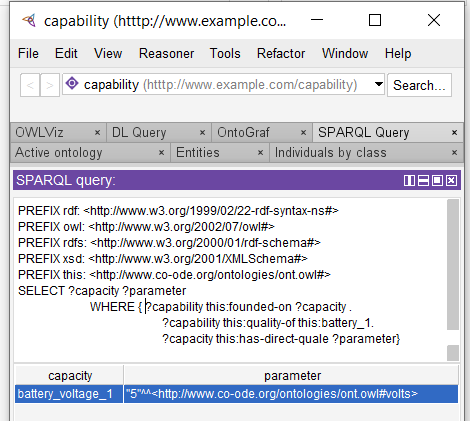
\includegraphics[width=0.45\textwidth]{query_screenshot.PNG}
  \caption{\label{fig:screen_query}}
\end{figure}

\begin{figure}
  \centering
  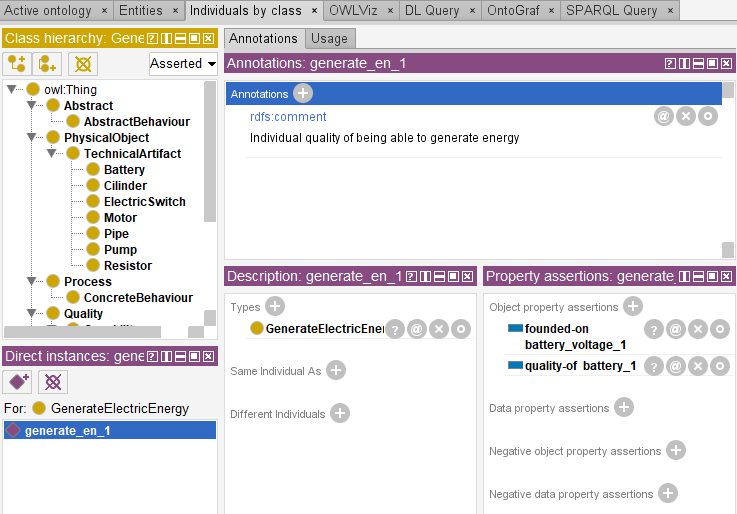
\includegraphics[width=0.45\textwidth]{entities_screenshot.PNG}
  \caption{\label{fig:screen_entities}}
\end{figure}

\section{Conclusion}\label{sec:conc}
\TODO{Riassumere cio' che e' stato detto nell'articolo.} %Ribadirne utilita'
\TODO{This work contributes towards a more precise understanding of fundamental concepts used in engineering, in particular functionality.
In particular, we have shown how one can give ontologically-grounded definitions capability, capacity, behavior and function using first order logic.
Moreover, we have shown how one can use functional decomposition to distinguish between ontological and engineering functions and, thereby, between capabilities and capacities.
Finally, we partially translated our first order theory in \OWL in order to show a preliminary serialisation of our theory in a computer-friendly formal language.}


%\begin{figure}[t]
%\includegraphics{}
%\caption{Figure caption.}\label{f1}
%\end{figure}

%\begin{table*}
%\caption{} \label{t1}
%\begin{tabular}{lll}
%\hline
%&&\\
%&&\\
%\hline
%\end{tabular}
%\end{table*}

\section*{Acknowledgemnts}

%%%% NOTA:
%Tutte le pubblicazioni scientifiche eventualmente prodotte dal/dalla 
%dottorando/a che usufruisce della borsa finanziata dalla presente 
%Convenzione e derivate dall'attività svolta nell'ambito del ciclo 
%di dottorato, oltre a indicare l'afferenza al Dottorato dell'Università,
%dovrà citare il sostegno all'attività di ricerca da parte del Finanziatore.

Francesco Compagno is funded
by the company Adige Spa.

%%%%%%%%%%% The bibliography starts:

%%%%%%%%%%%%%%%%%%%%%%%%%%%%%%%%%%%%%%%%%%%%%%%%%%%%%%%%%%%%%
%%                  The Bibliography                       %%
%%                                                         %%
%%  ios1.bst will be used to                               %%
%%  create a .BBL file for submission.                     %%
%%                                                         %%
%%                                                         %%
%%  Note that the displayed Bibliography will not          %%
%%  necessarily be rendered by Latex exactly as specified  %%
%%  in the online Instructions for Authors.                %%
%%                                                         %%
%%%%%%%%%%%%%%%%%%%%%%%%%%%%%%%%%%%%%%%%%%%%%%%%%%%%%%%%%%%%%


%\nocite{*}
% if your bibliography is in bibtex format, use those commands:
\bibliographystyle{ios1}           % Style BST file.
\bibliography{bibliography}        % Bibliography file (usually '*.bib')

% or include bibliography directly:
%\begin{thebibliography}{0}
%\bibitem{r1} F. Author, Information about cited object.
%
%\bibitem{r2} S. Author and T. Author, Information about cited object.
%\end{thebibliography}

\end{document}
